\documentclass[fancy, masters]{byuthesis}
% Class options are simple/fancy and masters/phd.
% Leave options blank for defaults.
% Defaults are simple for document style, and masters for degree type.


%%%%%%%%%%%%%%%%%%%%%%%%%%%%%%%
% Custom options and packages %
%%%%%%%%%%%%%%%%%%%%%%%%%%%%%%%
% Define path to figure files
\graphicspath{{figures/}}

% Define sequences of Latin text to fill space in example documents
% (not needed for your thesis -- delete or comment out if you'd like)
\usepackage{blindtext}


%%%%%%%%%%%%%%%%%%%%%%%%%%%%%%
% Define title page elements %
%%%%%%%%%%%%%%%%%%%%%%%%%%%%%%
% Thesis title for required BYU title page
\title{Forecasting Ride-hailing Across\\
\hspace*{0.333em}Multiple Model Frameworks}

% On the custom title page, use the same title, but format as you like
\customtitle{Forecasting Ride-hailing Across\\
\hspace*{0.333em}Multiple Model Frameworks}

% Your name goes here:
\author{Christopher Stephen Day}

% This is the date of graduation
\date{April 2021}

% If your degree is not a PhD or MS, then you can overwrite the degree using
\degree{Master of Science}

% Your department
\department{Department of Civil and Construction Engineering}

% The names of your committee members
\committeechair{Gregory S. Macfarlane}
  \committeemember{Grant G. Schultz}
  \committeemember{Gustavious P. Williams}

% Include any keywords you would like for your thesis/dissertation
\keywords{ride-hailing, activity-based model, multi-agent simulation, ActivitySim, BEAM, tour mode, tour purpose}


%%%%%%%%%%%%%%%%%%%%%%%%%%%%%%%%%%
% ---Bibliography source file--- %
%%%%%%%%%%%%%%%%%%%%%%%%%%%%%%%%%%
	\usepackage{algorithm}
\usepackage{algpseudocode}
\usepackage{dsfont}
\usepackage{pdflscape}
\usepackage{rotating}
\usepackage{float}
\usepackage{graphicx}
\usepackage{mathtools}
\usepackage{eqparbox}
\usepackage{makecell}
\usepackage{pgf}
	\usepackage{booktabs}
\usepackage{longtable}
\usepackage{array}
\usepackage{multirow}
\usepackage{wrapfig}
\usepackage{float}
\usepackage{colortbl}
\usepackage{pdflscape}
\usepackage{tabu}
\usepackage{threeparttable}
\usepackage{threeparttablex}
\usepackage[normalem]{ulem}
\usepackage{makecell}
\usepackage{xcolor}


%%%%%%%%%%%%%%%%%%%%%%%%%%%%%%%%%%
% ---Bibliography source file--- %
%%%%%%%%%%%%%%%%%%%%%%%%%%%%%%%%%%
%  Default is references.bib
\bibliography{}

\newlength{\cslhangindent}
\setlength{\cslhangindent}{1.5em}
\newlength{\csllabelwidth}
\setlength{\csllabelwidth}{3em}
\newlength{\cslentryspacingunit} % times entry-spacing
\setlength{\cslentryspacingunit}{\parskip}
% for Pandoc 2.8 to 2.10.1
\newenvironment{cslreferences}%
  {}%
  {\par}
% For Pandoc 2.11+
\newenvironment{CSLReferences}[2] % #1 hanging-ident, #2 entry spacing
 {% don't indent paragraphs
  \setlength{\parindent}{0pt}
  % turn on hanging indent if param 1 is 1
  \ifodd #1
  \let\oldpar\par
  \def\par{\hangindent=\cslhangindent\oldpar}
  \fi
  % set entry spacing
  \setlength{\parskip}{#2\cslentryspacingunit}
 }%
 {}
\usepackage{calc}
\newcommand{\CSLBlock}[1]{#1\hfill\break}
\newcommand{\CSLLeftMargin}[1]{\parbox[t]{\csllabelwidth}{#1}}
\newcommand{\CSLRightInline}[1]{\parbox[t]{\linewidth - \csllabelwidth}{#1}\break}
\newcommand{\CSLIndent}[1]{\hspace{\cslhangindent}#1}

\providecommand{\tightlist}{%
  \setlength{\itemsep}{0pt}\setlength{\parskip}{0pt}}

%%%%%%%%%%%%%%%%%%%%%%%%%%
% --- Begin Document --- %
%%%%%%%%%%%%%%%%%%%%%%%%%%
\begin{document}


%%%%%%%%%%%%%%%%%%%%%%%%%%%%%%%%%%%%%%%%%%%%%%%%%%%%%%%
% --- Front matter (probably don't need to change)--- %
%%%%%%%%%%%%%%%%%%%%%%%%%%%%%%%%%%%%%%%%%%%%%%%%%%%%%%%
	\frontmatter

	\titlepage
	\clearpage

	\customtitlepage
	\clearpage


    \begin{abstract}
  The advent of on-demand transport modes such as ride-hailing and microtransit has challenged forecasters to develop new methods of forecasting the use and impacts of such modes. In particular, there is some professional disagreement about the relative role of activity-based transportation behavior models --- which have detailed understanding of the person making a trip and its purpose --- and multi-agent demand simulations which may have a better understanding of the availability and service characteristics of on-demand services. A particular question surrounds how the relative strengths of these two approaches might be successfully paired in practice. Using daily plans generated by the activity-based model ActivitySim as inputs to the BEAM multi-agent simulation, we construct nine different methodological combinations by allowing the choice to use a pooled ride-hail service in ActivitySim, in BEAM with different utility functions, or in both. Within each combination, we estimate ride-hailing ridership and level of service measures. The results suggest that mode choice model structure drastically affects ride-hailing ridership and level of service. In addition, we see that multi-agent simulation overstates the demand interest relative to an activity-based model, but there may be opportunities in future research to implement feedback loops to balance the ridership and level of service forecasts between the two models.
  \end{abstract}
  	\clearpage


    \begin{acknowledgments}
  I would first like to acknowledge my advisor and friend, Dr.~Gregory Macfarlane, for teaching me everything I know. Without you, this thesis and my future career would be boring and stupid. I found a work to love and enjoy while researching under your supervision, and for that I will forever be grateful. I express gratitude as well to Dr.~Schultz and Dr.~Williams for being on my advisory committe and helping me finish my thesis. I would also like to acknowledge the United States Department of Transportation (USDOT) for funding my research. Thank you to the members of the T-SCORE center, especially Dr.~Gregory Erhardt, Jawad Hoque, and Vedant Goyal for their friendship and assistance with tackling BEAM. A special shoutout to Nate Lant and Hayden Atchley for working on ActivitySim and BEAM even when we had no idea what we were doing. Together, we got this thing done. I am enormously grateful as well to Zachary Needell at Lawrence Berkeley National Laboratory for working with the T-SCORE team and me in our efforts to tame BEAM. Without you, none of this would have been possible. An additional thanks to Wasatch Front Regional Council, especially Chad Worthen, for sharing data and working with our group. Also, a standing ovation to the creators of the ggalluvial R package; this package is awesome and allowed me to make some pretty cool plots.

  I express sincere gratitude for my family members and their patience and support as I conducted this research. Especially, thank you to my wife Megan, because without her I would probably be dead. She convinced me to apply for this research position, held down the fort at home, let me work every Saturday for 3 years, and was patient with me everytime I went insane staring at my computer screeen. I appretiate you all. Finally, thank you to the BYU tennis courts and Kevin Lunt, because tennis is the key to happiness.
  \end{acknowledgments}
  	\clearpage

	\tableofcontents*
	\clearpage

	\listoffigures
	\clearpage

	\listoftables
	\clearpage

	\nomenclature{$c$}{Speed of light in a vacuum inertial frame}
\nomenclature{$h$}{Planck constant}
\nomenclature{$\mathit{Re}$}{Reynolds number}
\nomenclature{$\mathbf{x}$}{State vector}
\nomenclature{$\alpha$}{Angle of attack}
\nomenclature{$\beta$}{Sideslip angle}
\nomenclature{$\gamma$}{Climb angle}
\nomenclature{$p$}{Roll rate}
\nomenclature{$q$}{Pitch rate}
\nomenclature{$r$}{Yaw rate}
\nomenclature{$P$}{Covariance matrix}

\printnomenclature
	\clearpage

%%%%%%%%%%%%%%%%%%%%%
% --- Main Body --- %
%%%%%%%%%%%%%%%%%%%%%
	\mainmatter

\hypertarget{intro}{%
\chapter{Introduction}\label{intro}}

\hypertarget{problem-statement}{%
\section{Problem Statement}\label{problem-statement}}

On-demand transit modes, such as microtransit and ride-hailing, can make private car-centric societies more sustainable (Tirachini, 2020). They have the potential to exhaust less vehicular emissions, decrease roadway congestion, increase health, increase public transit usage in some cases, and be economically viable (Chen et al., 2021; Marquet, 2020). As urban centers attempt to shift from a private car-centric environment to a multi-modal system, forecasters are challenged with modeling accurate ridership and level of service values. Since ride-haling is already heavily involved in today's transportation system, estimating the uptake of ride-hailing usage and understanding the service capabilities of ride-hailing is critical to a sustainable future.

Unfortunately, forecasting the ridership and level of service of ride-hailing and other novel modes is a challenging feat with no clear methodological approach. Individuals using ride-hailing vehicles behave differently than when using regular car modes and so understanding their behavior and the ride-hailing service capabilities is particularly challenging (Dean \& Kockelman, 2021; X. Dong, 2020; Kang et al., 2021; Y. Li et al., 2020). In addition, the ridership of bike share, an affordable and sustainable bike rent program, has been modeled many times each with a different methodology (Biehl et al., 2019; Cho \& Shin, 2022; Hyland et al., 2018; Li \& Kamargianni, 2018; Song et al., 2019; Welch et al., 2020; Zhou et al., 2019). Similarly, forecasters have struggled to find the best technique for estimating the ridership of e-scooters (public electric scooters) and in what locations they would be most effective (Hosseinzadeh et al., 2021; H. Lee et al., 2021a; M. Lee et al., 2021b; Tuli et al., 2021; W. Zhang et al., 2021; Zuniga-Garcia et al., 2022).

Many different modeling methodologies exist with the purpose of better understanding the behavior of individuals using ride-hailing vehicles and other novel modes. For example, some forecasters use activity-based models, which construct daily activity patterns to model individual travel behavior, to better understand the travel patterns of those who use novel modes (Macfarlane et al., 2021; Muhammad et al., 2019; Xu et al., 2019). Other forecasters use multi-agent simulation, which focuses on modeling the interactions between different agents, to understand the level of service of transport technologies (Hörl et al., 2019b; Sánchez et al., 2019; Shimizu et al., 2013). Some use spatial analysis joint with geography data to better understand where individuals use novel modes, like pickup and drop off locations, to travel (Cho \& Shin, 2022; Hosseinzadeh et al., 2021; Hyland et al., 2018). Zhou et al. (2019) have even attempted to use machine learning techniques to determine the optimal mode choice between bike-sharing and taxi services. Among these, and the other strategies that exist, some professional disagreement exists as to which approach would best serve forecasters in their efforts to model the ridership and level of service of ride-hailing to create sustainable city centers. In particular, a lack of understanding exists whether the relative strengths of an activity-based model and multi-agent simulation could be paired together successfully to model the uptake of on-demand services.

\hypertarget{scope-within-t-score}{%
\section{Scope within T-SCORE}\label{scope-within-t-score}}

In 2020, a project from the Transit - Serving Communities Optimally, Responsively, and Efficiently (T-SCORE) Center was proposed with the goal of keeping transit sustainable and resilient into the future. As a result T-SCORE was divided up into two tracks: the community analysis track and the multi-modal optimization and simulation (MMOS) analysis track. The MMOS analysis track had the purpose of using modeling techniques to determine the effectiveness of on-demand transit modes and their efficiency at bringing users to and from transit locations. The hypothesis was that instead of having ridership of public transit compete with ride-hailing, to instead pair together ride-hailing and transit services. Modeling ride-hailing vehicles was an effective avenue toward understanding their impact on transit ridership. Figure \ref{fig:mmos} shows the entire modeling and optimization process used in the MMOS track to analyze ride-hailing vehicles. The inputs are represented in green whereas the outputs are represented in yellow (with the exception of the mode choice model). The ideas behind this research originated with an attempt to develop an optimal mode choice model structure to forecast ride-hailing service capabilities for the T-SCORE project.

\begin{figure}

{\centering 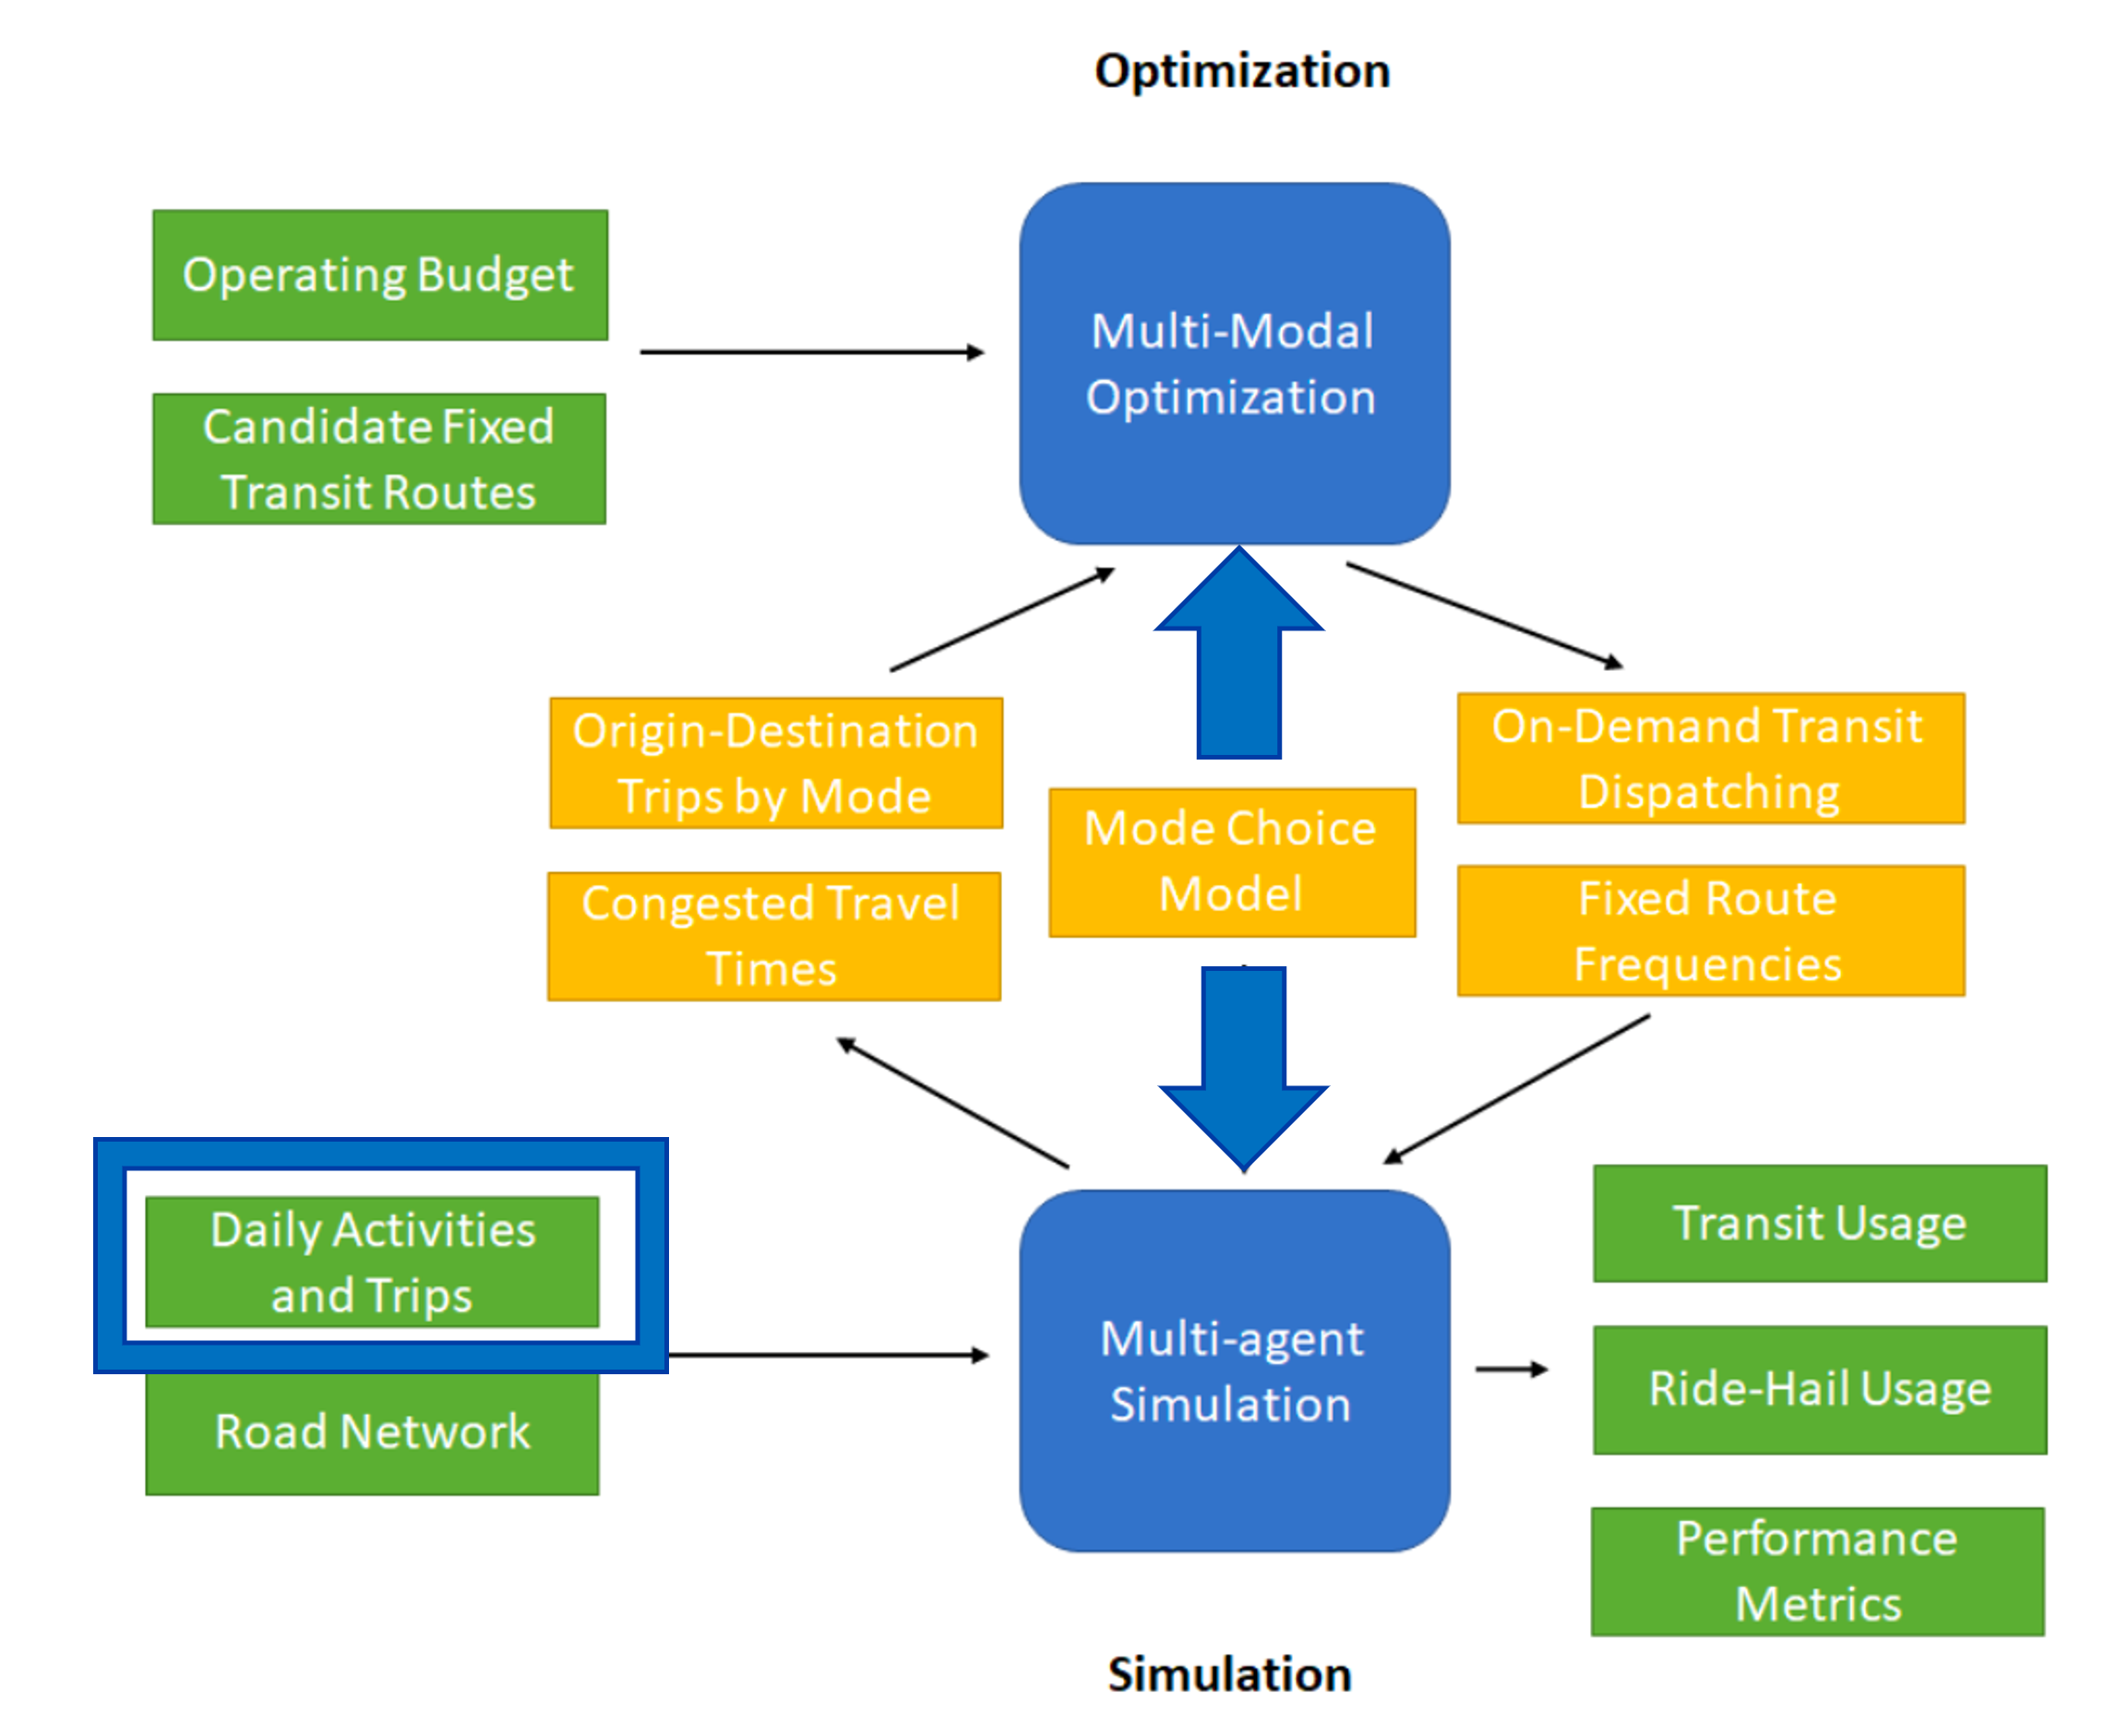
\includegraphics[width=0.75\linewidth]{pics/mmos_mode} 

}

\caption{Overview of the T-SCORE MMOS tract process.}\label{fig:mmos}
\end{figure}

\hypertarget{purpose-of-research}{%
\section{Purpose of Research}\label{purpose-of-research}}

We develop a series of experiments to understand the relative importance of a paired activity-based model and multi-agent simulation in forecasting the use of ride-hailing services. We do this by examining the ridership and level of service of ride-hailing predicted by different activity-based model and multi-agent simulation mode choice combinations. Specifically, we use the daily activity plans generated by ActivitySim as inputs to the multi-agent simulation BEAM to establish nine different combinations of methodolgical approach. For each methodological combination, we estimate ride-hailing ridership and level of service outputs for a Salt Lake City, Utah case study region. The purpose of this research is not, however, a test of model accuracy in estimating ride-hailing ridership and level of service but instead, a in-depth comparison between different modeling approaches. With this comparison we aim to understand the relative effect different paired mode choice combinations can have in forecasting ride-hailing services.

Section \ref{lit} presents a brief literature review on different methodological approaches used to forecast ride-hailing services. Our specific methodological approach is then explained in Section \ref{meth} with our results explained thereafter in Section \ref{results}. A discussion on our results along with limitations and further research ideas are presented in Section \ref{discussion}. The paper also concludes with a summary of our findings in Section \ref{discussion}.

\hypertarget{lit}{%
\chapter{Literature Review}\label{lit}}

As discussed in the Introduction, forecasters have modeled the level of service and the individual travel behavior of ride-hailing and other novel modes in a variety of ways. To best understand a few of the methodological approaches forecasters have used, the following literature review outlines the pros and cons of using spatial analysis, activity-based models, multi-agent simulation, and paired modeling approaches to model the use and impacts of ride-hailing. Since those individuals who use novel modes in general have similar travel behavior to those who use ride-hailing, we include references to research about both ride-hailing services and other novel modes.

\hypertarget{lit-simp}{%
\section{Spatial Analysis and Ride-hailing}\label{lit-simp}}

The most prominent methodological approach to understanding ride-hailing service is through simple approaches like spatial, statistical, and empirical analyses. For example Correa et al. (2017) developed heatmaps using spatio-temporal data to analyze ride-hailing pickup locations. Marquet (2020) processed data and used statistical measures to estimate a connection between walkability index and ride-hailing usage. Y. Dong et al. (2018) conducted an empirical analysis to understand the unique travel patterns of ride-hailing vehicles. Many other research studies have used simple approaches to estimate the ridership and service of ride-hailing and other novel modes (Cho \& Shin, 2022; Hosseinzadeh et al., 2021; Hyland et al., 2018; Li et al., 2022; Zhou et al., 2019).

The upside to implementing a simple spatial, statistical, or empirical analysis is its simplicity. The downside, however, is that with its simplicity comes decreased flexibility. For example, Hosseinzadeh et al. (2021) determined regional attributes that affect the density of regional e-scooter trips by conducting a spatial analysis. By following a simple statistical approach they learned of the impact land use, age, and other demographics have on e-scooter use, but did not have the flexibility to understand e-scooter travel times and other level of service measures. Also, simple spatial, statistical, and empirical methods oftentimes only answer one particular geographic question. For example, Li et al. (2022) estimated a correlation between the number of ride-hailing pickup and drop-offs with the location of subway services and transit routes. Although these results may provide insights on how to improve transit services, ride-hailing level of service and ridership statistics could not be estimated as well. Overall, spatial, statistical, and empirical analyses are unable to accurately forecast the ridership, level of service, and other usage measures simultaneously.

\hypertarget{lit-abm}{%
\section{Activity-based Models and Ride-hailing}\label{lit-abm}}

Activity-based models are transportation behavior models that construct daily activity patterns for synthetic individuals from behavioral choice models. Activity-based models predict the set of activities to participate in before they predict how and when to get to those activities (Philip et al., 2013). By estimating activity demand before mode choice and route selection, activity-based models more accurately represent the way people travel. Activity-based models also use utility theory and logit based regression to best estimate individual decisions and travel behavior (Bowman, 1998). In addition to representing behavior accurately, another advantage to using activity-based models is the modal consistency between trips on the same tour (Gomes et al., 2021; Hasnine \& Nurul Habib, 2021; Knapen et al., 2021; Nayak \& Pandit, 2022). In other words, activity-based models ensure that individuals choose coherent modes between subsequent trips (modal consistency) when those trips occur on the same tour (a sequence of trips starting and ending at the home location). In real life, individuals travel in a similar manner among trips of the same tour. Activity-based models account for this natural tendency by chaining trips of the same individual together, or by developing a tour mode construct. A tour mode represents the primary mode any particular person selects to use on a tour. By estimating individual behavior accurately and by maintaining modal consistency among trips of the same individual, ride-hailing usage can be consistently distributed to the same trips and same individuals in activity-based models, suggesting justifiable ride-hailing selection estimates.

Many forecasters elect to use activity-based models to model ride-hailing and other modes because of the behavioral representation and modal consistency they provide. For example, Nguyen et al. (2022) modeled one-way car-sharing services with an activity-based model because the modal consistency between trips allowed them to estimate vehicle usage. Xu et al. (2019) modeled privately-owned autonomous vehicles with an activity-based model as a way to better understand their impact on household travel patterns. Rafiq \& McNally (2022) used an activity-based approach to estimate the five most common tour structures of ride-hailing individuals. Activity-based models can determine the specific travel patterns of those who use ride-hailing services.

Although there are advantages to using activity-based models to model ride-hailing, forecasters must consider the various weaknesses that exist when using activity-based models. One of the biggest shortfalls with most activity-based models is that travel times are averaged along travel links (Mahmoudi et al., 2021; RSG, 2016). For example, although Nguyen et al. (2022) used an activity-based model to model one-way car sharing, they noted that it used a regression function to estimate travel time. For this reason, Nguyen et al. (2022) noted that it was more difficult to verify the service capabilities of the car-sharing modes. Many activity-based models also use pre-generated skims composed of average travel statistics to determine service related measures (L. Zhang et al., 2018). Skims are large matrices composed of travel time, distance, and cost that exist between every origin-destination zone combination. With a dynamic traffic assignment (DTA) model, travel statistics between every origin-destination zone are determined by spatially aggregating each zone and then by calculating average values between the centroid of each zone using a loaded network-assignment methodology. Activity-based models lack variability when modeling travel and wait times of ride-hailing and other novel vehicles because they use travel skims as a primary input. In addition, since concrete travel values are used as inputs, it can be difficult to model ride-hailing vehicle availability and passenger capacity limitations.

\hypertarget{lit-mas}{%
\section{Multi-agent Simulation and Ride-hailing}\label{lit-mas}}

An alternative to activity-based models for forecasting ride-hailing level of service is multi-agent simulation. Multi-agent simulation models interactions between individual agents by reading in a set of detailed daily activity patterns onto a transportation network (Amblard et al., 2015; Bazghandi, 2012; Siebers \& Aickelin, 2008). Some multi-agent simulations also use an iterative process to maximize the individual travel utility by achieving mode, route, and overall traffic equilibrium. By forecasting travel behavior on an individual level until equilibrium is reached, varied, reasonable wait time and travel time estimations are predicted for every agent. Forecasting level of service with unique travel time statistics produces more realistic results. Along with modeling each individual closely, a multi-agent simulation keeps track of every ride-hailing vehicle as well. The complexity of the vehicular availability model along with individual travel behavior model allows multi-agent simulation to estimate exact, variable wait and travel times. For example, the model knows the exact ride-hailing vehicle availability and ride-hailing passenger capacity at every moment of the day. Therefore, capacity measures, like ride-hailing ridership and utilization, can be estimated realistically and with great precision at the individual level using multi-agent simulation.

Various forecasters elect to use multi-agent simulation to model the level of service of ride-hailing and other novel modes because agent-to-agent and agent-to-vehicle interactions are modeled closely. For example, Kamel et al. (2019) chose to use a multi-agent simulation to model shared autonomous vehicles (SAVs) because the granularity of the interaction between different agent types and SAV modes helped the researchers understand the effect user preference has on modal decisions. Hörl et al. (2019b) also analyzed shared autonomous vehicles with a multi-agent simulation, mainly to take advantage of the detailed vehicular model. The model allowed forecasters to adjust fleet size and to optimize the way fleet vehicle drivers behaved. By utilizing the advanced vehicular model, the researchers were able to estimate the overall system performance, wait times, and cost of various autonomous vehicle fleets. Similarly, Becker et al. (2020) used MATSim, an open source agent-based simulation used for large scale scenarios, to model the travel times and costs of different on-demand transit modes (ride-hailing, car-sharing, bike-sharing) (W Axhausen et al., 2016). The primary advantage of MATSIM is that it provides a ``dynamic demand response towards changes in service attributes such as travel times or costs'' (Becker et al., 2020). Many forecasters continue to analyze new transportation technologies with multi-agent simulation because its inherit advantages are helpful to understanding service capabilities.

Although multi-agent simulation excels at estimating the level of service of ride-hailing vehicles at fine detail, various pitfalls do exists. For example, Ciari et al. (2016) summarizes a multitude of research done to understand demand for car-sharing with the multi-agent simulation MATSim. In this research, they note that although multi-agent simulation provides an extensive level of detail, it does not necessarily equate to real world accuracy. Because MATSim uses an iterative process of maximizing individual utility until a state of overall equilibrium is reached, it remains difficult to accurately portray exact individual behavior choices (Ciari et al., 2016). The structure of the activity-based choice model allows strong individual behavioral representation, whereas the complexity of the multi-agent simulation may cause individual choices to be inaccurate and unreasonable. Similarly, where the activity-based model may excel at more realistic mode choice selections among trips of the same tour, some multi-agent simulation struggle. For example, Figure \ref{fig:fig-mode-compare} provides a visual example of mode choice shortcoming present in some multi-agent simulations. As seen in Figure \ref{fig:fig-mode-compare}, all trips of the same tour for the activity-based model are based on the selected tour mode. This allows users to switch from one mode to another between trips, as long as they are compatible. On the other hand, the multi-agent simulation may only undergo mode choice selection on the first trip of the tour, and be trapped into using that same mode on future trips. This is not true for all multi-agent simulations, but is true for the multi-agent simulations most often used in the literature. This results in less realistic travel behavior. The last inherit weakness of multi-agent simulation is that it is computationally heavy; requiring abundant time and resources. Overall where the multi-agent simulation lacks in forecasting ride-hailing services the activity-based model excels, and vice versa, and so the combination of using both strategies could prove effective.

\begin{figure}

{\centering 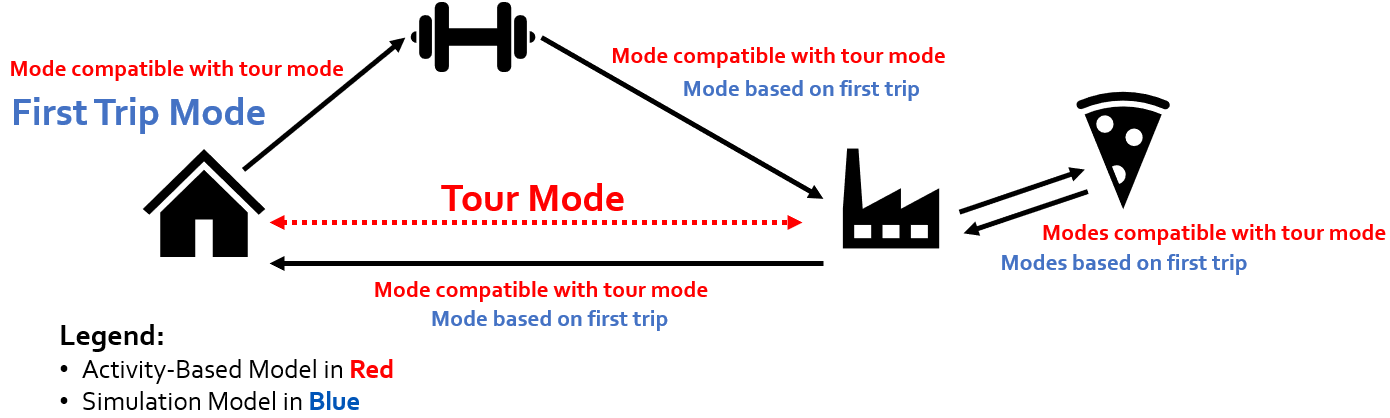
\includegraphics[width=1\linewidth,]{pics/abm-mas-compare} 

}

\caption[Activity-based models vs. multi-agent simulation.]{Mode choice in activity-based models and multi-agent simulation.}\label{fig:fig-mode-compare}
\end{figure}

\hypertarget{limited-attempts-to-pair-mulitple-modeling-approaches}{%
\section{Limited Attempts to Pair Mulitple Modeling Approaches}\label{limited-attempts-to-pair-mulitple-modeling-approaches}}

The varying strengths and weaknesses within both activity-based models and multi-agent simulation point to possibly using both approaches to understand ride-hailing ridership and level of service. Yet few forecasters have attempted to reconcile or pair these two disparate approaches in order to better understand the behavior of ride-hailing and other novel modes. However, one example of reconciling the traditional approaches is with the Microsimulation Transport Orchestrator (MITO) system (Moeckel et al., 2020; Zwick et al., 2021). MITO's primary purpose is to overcome the limitations of the traditional trip-based model while being easier to implement than the traditional activity-based model. Like an activity-based model, MITO simulates each agent individually. MITO also includes a simplified activity schedule builder, allows forecasters to add attributes, allows agent tracing, and is not as computationally heavy as traditional multi-agent simulations (Moeckel et al., 2020). Zwick et al. (2021) used MITO to estimate travel demand and MATSim to simulate that demand. By pairing together MITO and MATSim, the researchers were able to gather service criteria for pooled on-demand ride-hailing vehicles at a detailed level, while also maintaining the behavioral integrity of each agent.

Another example of pairing together two disparate modeling approaches involves discrete choice and MATSIM. Since MATSim implements a feedback loop to determine mode choice instead of using a discrete choice model, some researches have attempted to pair together a discrete mode choice model with MATSim in attempt to shorten the number of iterations needed to be run. For example, Hörl et al. (2019a) discovered that by using a discrete choice model within MATSim, no irrelevant mode choice decisions were made. This indeed, lead to less iterations being run while enhancing the realistic nature of the mode choice selection. However, although initial modal decisions were more accurate than the default MATSim model, the discrete choice model added a layer of complexity. The need for more accurate and useful data gave the model runners less freedom.

\hypertarget{summary}{%
\section{Summary}\label{summary}}

Overall, these few examples show that by pairing together multiple model frameworks the strengths of each model can be maximized. To the authors knowledge, however, no previous literature exists on pairing together an activity-based model and a multi-agent simulation for the purpose of modeling ride-hailing ridership and level of service. By using an activity-based model we hope to take advantage of the strong individual behavior representation and realistic mode choice decisions. By using a multi-agent simulation we hope to take advantage of the vast individual travel behavior detail and the advanced vehicular availability model. We therefore hypothesize that with a joint activity-based model and multi-agent simulation, we can utilize the advantages of both models to capture ride-hailing ridership and level of service measures. However, question remains as how to pair together both models with the purpose of forecasting ride-hailing ridership and level of service. And so, in this research we explore different linked activity-based model and multi-agent simulation mode choice combinations to understand the affect each one has on the usage of ride-hailing modes. We aim to answer the question, ``Does the setup of a linked activity-based model and multi-agent simulation mode choice model structure matter?''

\hypertarget{meth}{%
\chapter{Methods}\label{meth}}

We developed a series of experiments to understand the relative importance of pairing an activity-based and multi-agent simulation in forecasting the uptake of ride-hailing. We performed these experiments using ActivitySim as the activity-based model and BEAM as the multi-agent simulation. We used the Salt Lake City, Utah region as a case study for our experiments. The following section outlines the methodology for which we were able to model ride-hailing ridership and level of service with differing activity-based model and multi-agent simulation mode choice combinations.

\hypertarget{ride-hailing-in-activitysim}{%
\section{Ride-hailing in ActivitySim}\label{ride-hailing-in-activitysim}}

We chose ActivitySim as the activity-based model in this research because it is an open-source software with ride-hailing modal alternatives built into its framework (ActivitySim, 2021). Specifically, the ride-hail mode and the pooled ride-hail mode fall under one of the four nested tiers of ActivitySim's nested logit mode choice model. This means that ride-hail is a unique modal option not characterized by being an auto, non-motorized, or transit type mode. Figure \ref{fig:fig-asim-nest} displays the four tiers of the nested logit mode choice model along with the modal alternatives of each tier (MTC, 2012). These modal alternatives represent the alternatives available in both ActivitySim's tour based and trip based mode choice model. When determining the mode to use on a trip, ActivitySim first calculates the tour mode and subsequently calculates the trip mode based on the tour mode selection (See Figure \ref{fig:fig-mode-compare}). Person attributes, path attributes, location attributes, tour purpose value (the main activity purpose of the tour), and more all play a role in calculating the mode choice decision.

\begin{figure}

{\centering 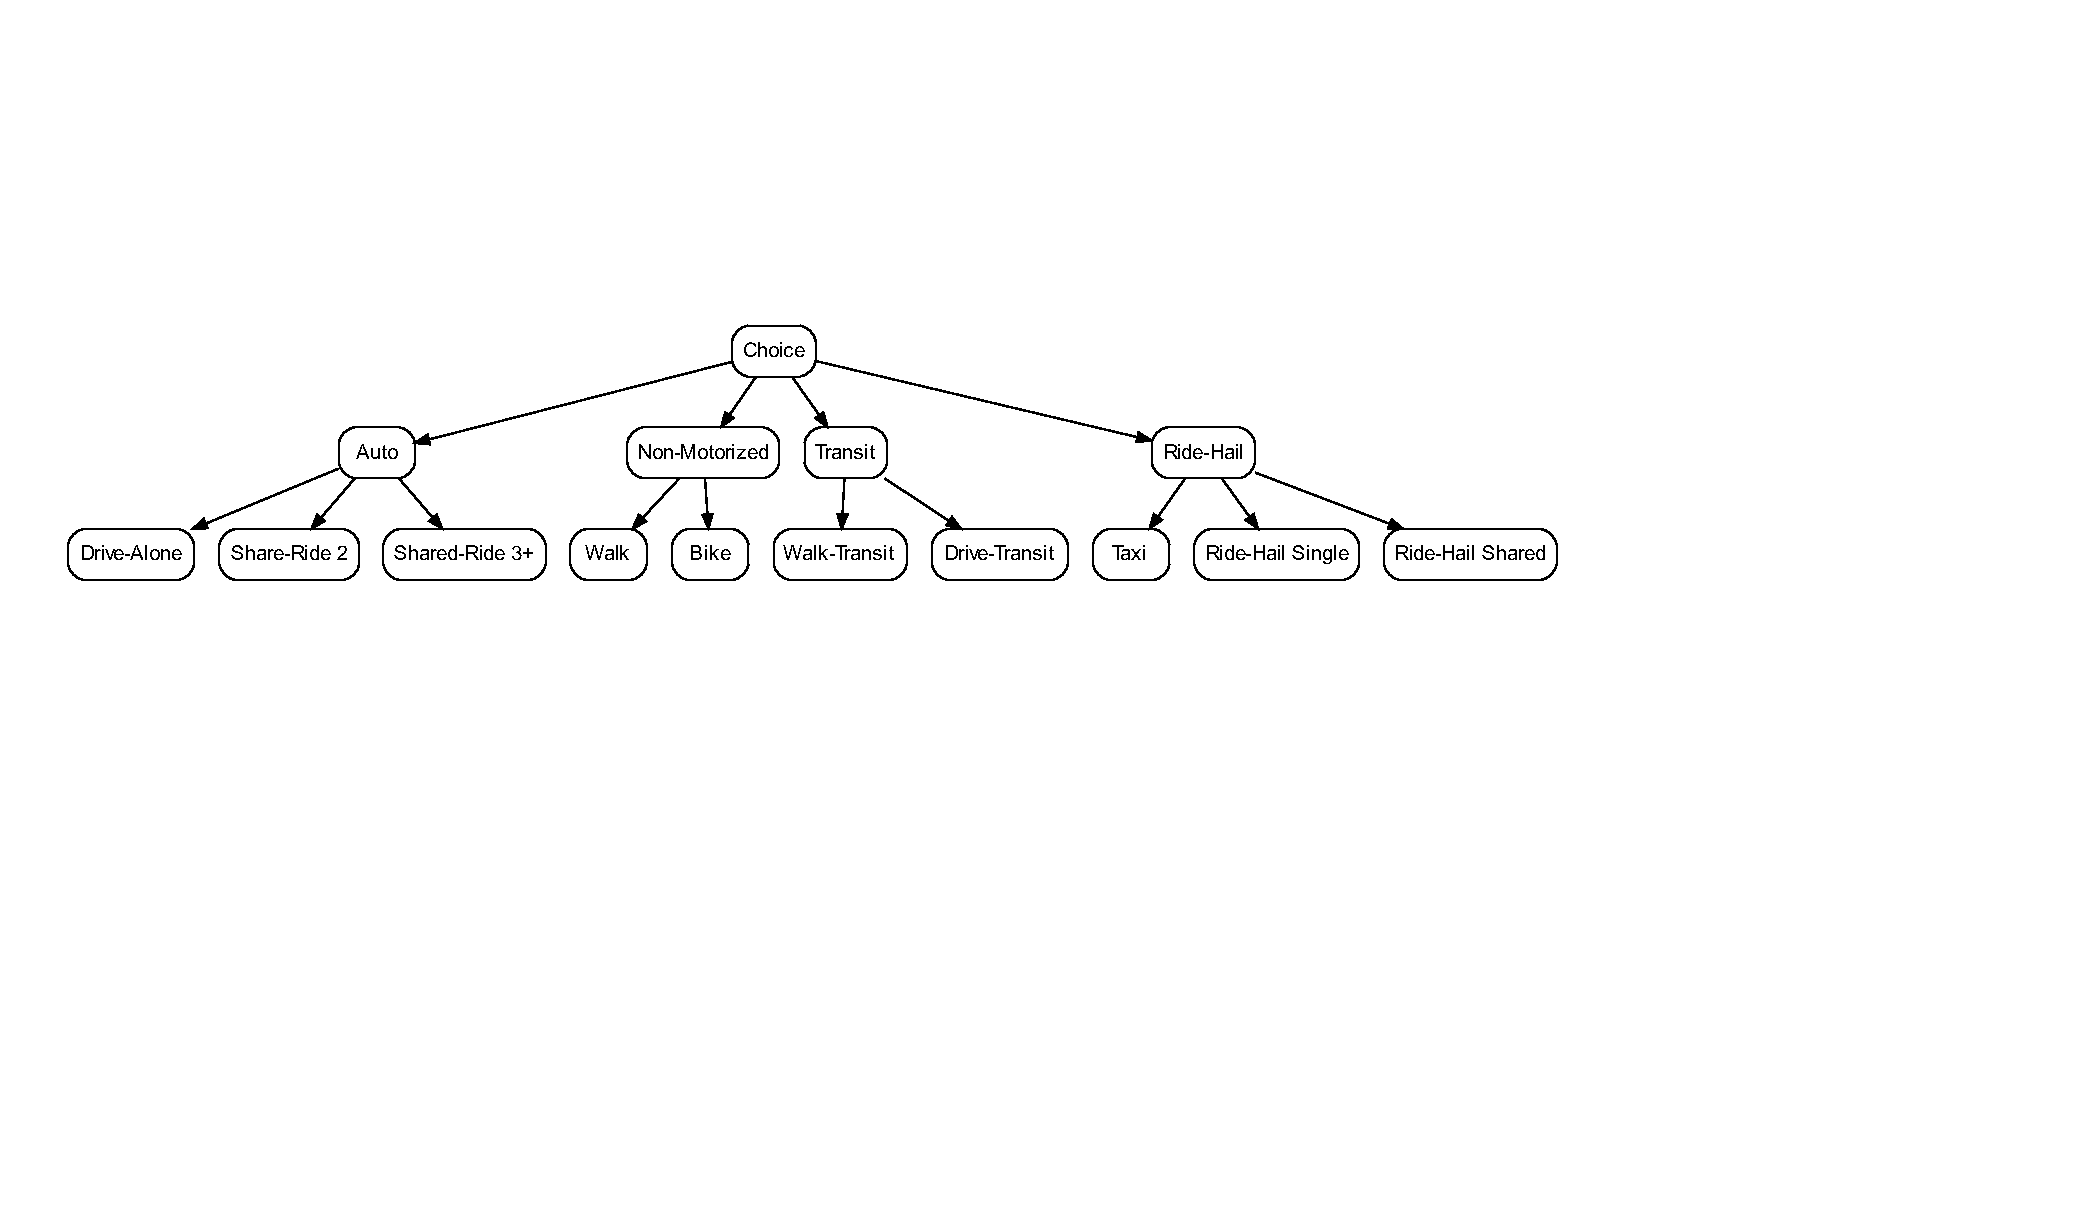
\includegraphics[width=1.6\linewidth,trim = {1cm 9.5cm 4.5cm 6cm}]{thesis_files/figure-latex/fig-asim-nest-1} 

}

\caption{Nested logit model used in ActivitySim.}\label{fig:fig-asim-nest}
\end{figure}

In ActivitySim, the utility \(V\) for person \(n \in {1:N}\) choosing alternative mode \(k \in K\) between origin zone \(i \in I\) and destination zone \(j \in J\) is:

\begin{align}
  V_{nk}^{Person} =& \ \alpha_{kn} + \beta_{kP}^1(cost_{k,ij}) + \beta_{kP}^2(age_{n}) 
   + \beta_{kP}^3(hhsize_{n}) \label{eq:person} \\
  V_{nk}^{Path} =& \ \beta_{kP}^4(dist_{k,ij}) +  \beta_{kP}^5(tv_{k,ij}) + 
       \beta_{kP}^6(te_{k}) +  \beta_{kP}^7(tw_{k}) + \nonumber \\ 
      & \ \beta_{kP}^8(prox_{k}) + \beta_{kP}^9(xfer_{k})  \label{eq:path} \\
  V_{nk}^{Location} =&  \ \beta_{kP}^{10}(ZDI_{k,i}) + \beta_{kP}^{11}(ZDI_{k,j}) + 
      \beta_{kP}^{12}(ZTI_{k,j}) + \nonumber \\ 
      & \ \beta_{kP}^{13}(CBD_{k,j}) \label{eq:location}\\
  V_{nk} =& \ V_{nk}^{Person} + V_{nk}^{Path} + V_{nk}^{Location} \label{eq:all}
\end{align}
where, \(\alpha\) is the alternative specific constant that varies by auto sufficiency, \(hhsize\) is household size, \(dist\) is distance, \(tv\) is vehicle travel time, \(te\) is egress time, \(tw\) is wait time, \(prox\) is proximity to transit, \(xfer\) is number of transfers, \(ZDI\) is zonal density index, \(ZTI\) is zonal topography index, \(CBD\) is central business district, and \(\beta_{P}^1:\beta_{P}^{13}\) are estimated coefficients that vary by tour purpose \(P\). Equation \eqref{eq:person} shows part of the ActivitySim's mode choice utility function that focuses on person variables. Equation \eqref{eq:path} shows the part of the mode choice utility function that focuses on path variables. Equation \eqref{eq:location} shows the part of the mode choice utility function that focuses on location variables. As shown in Equation \eqref{eq:all}, ActivitySim uses the combination of person, path, and location variables to calculate the mode choice alternative. The combination of these different variable types determines whether or not a person selects a ride-hailing mode. In addition, since activity-based models do not use variable wait time, the average wait time is selected before the model run.

\hypertarget{configuring-activitysim}{%
\section{Configuring ActivitySim}\label{configuring-activitysim}}

ActivitySim requires three inputs:

\begin{enumerate}
\def\labelenumi{\arabic{enumi}.}
\tightlist
\item
  A synthetic population of the agents within the study area.
\item
  A zonal socioeconomic data file describing the characteristics of each zone.
\item
  A set of skims that describe the cost and travel times of all modes between all zones.
\end{enumerate}

We generated the synthetic population by inputting a seed table and a set of regional targets into PopulationSim (PopulationSim, 2021). We created the zonal socioeconomic file using data from Wasatch Front Regional Council (WFRC) (WFRC, 2019), Utah Automated Geographic Reference Center (AGRC, 2021), and the synthetic population when necessary. Finally we used travel time and cost skims that were pre-generated from WFRC (2019). For additional details relating to how the inputs were processed and gathered please refer to the research conducted by Macfarlane et al. (2021).

After generating the necessary input files, we calibrated and validated the ActivitySim model to better represent decisions made in the Salt Lake region. The process of calibrating and validating the ActivitySim model to the Salt Lake region was conducted by Macfarlane et al. (2021). The purpose of the calibration and validation was to ensure that the outputs generated by ActivitySim matched target regional values. Specifically, trip productions, trip distributions, and mode choices were tested to match the given target values provided in the four-step model from WFRC (2019). The details behind the exact calibration and validation process are discussed by Macfarlane et al. (2021), and therefore will not be described in detail.

\hypertarget{novel-beam}{%
\section{Ride-hailing in BEAM}\label{novel-beam}}

The Behavior, Energy, Autonomy, and Mobility (BEAM) model, developed by Lawrence Berkeley National Laboratory and UC Berkeley Institute for Transportation Studies, was chosen as the multi-agent simulation in this research (BEAM, 2022). As an extension of MATSim, it simulates individual agents using both within day replanning and across-day replanning to maximize individual utility. BEAM was mainly chosen as the multi-agent simulation in this research because of its integration with ride-hail and pooled ride-hail vehicles. Along with the ride-hailing type mode options, BEAM supports other mode options such as car, walk, bike, walk-to-transit, and drive-to-transit. The default BEAM version uses a simple multinomial logit mode model to determine which mode any particular agent will use on any particular trip. The default version of BEAM calculates the utility \(V\) for person \(n \in {1:N}\) choosing alternative mode \(k \in K\) between origin zone \(i \in I\) and destination zone \(j \in J\) as:

\begin{equation}
  V_{nk} = \alpha_{k} + \beta_k^1(cost_{k,ij}) + \beta_k^2(tv_{k,ij}) + \beta_k^3(xfer_{k}) \label{eq:beam}
\end{equation}
where, \(\alpha\) is the alternative specific constant that varies mode, \(tv\) is vehicle travel time, \(xfer\) is number of transfers and \(\beta_{P}^1:\beta_{P}^{3}\) are estimated coefficients that vary mode.

However, we improved the BEAM's default mode choice model in order to better estimate the ride-hailing choices of individuals. Specifically, we changed the BEAM mode choice model to use a tour purpose attribute, the same utility equations as ActivitySim (See Equation \eqref{eq:all}), and additional modal alternatives consistent with those present in ActivitySim. Appendix A provides a deeper explanation of these changes.

In addition to having a consistent mode choice structure with that of ActivitySim, BEAM implements ride-hailing vehicular behavior and assignment. BEAM uses a greedy asynchronous ride-hailing matching algorithm that also supports pooled trips (BEAM, 2022). The algorithm works by requiring agents to send a request for a ride-hail vehicle, and then by matching the closest vehicle available to that agent. For the algorithm to work, BEAM requires the modeler to input a ride-hail vehicle fleet. This fleet is a simple file that describes the number of ride-hail vehicles available in the region, their starting locations, their working hours, their seating capacity, and other specifications. Our fleet was generated by a student at Georgia Institute of Technology who used statistical models to predict fleet specifications. BEAM assigns fleet vehicles to the roadway network, where they ``roam'' the streets awaiting requests. The ride-hail algorithm permits a more realistic ride-hail modeling structure. For example, agents make a request to take a ride-hail vehicle, expect a variable wait time dependent on their geographic location, and may not even be able to take the vehicle if there is no availability. All these attributes are similar to how using ride-hailing is in real life, and represent the true advantages to modeling ride-hailing ridership and level of service with BEAM.

\hypertarget{configuring-beam}{%
\section{Configuring BEAM}\label{configuring-beam}}

BEAM was configured to the case study region by gathering the input data, validating the utility parameter values, and calibrating the utility alternative specific constants (ASC) to match regional totals. Most of the BEAM input files were directly generated by the calibrated ActivitySim model, with the exception of the network from WFRC (2019) and the General Transit Feed Specification (GTFS) data from Utah Transit Authority (2021). The utility parameter coefficients used in BEAM's mode choice model were copied directly from Metropolitan Transportation Commission's (MTC) implementation of ActivitySim (MTC, 2012). MTC's implementation of ActivitySim was designed for the San Francisco, California region. Logically, travel behaviors such as travel time, travel distance, and number of transfers should affect people in different regions in similar ways. However, as a way to validate the use of ActivitySim's path utility coefficients in the Salt Lake region, we compared these values to values from the Utah Statewide model (UDOT, 2021), the WFRC travel demand model (WFRC, 2019), and National Cooperative Highway Research Program (NCHRP) Report 716 (Cambridge Systematics et al., 2012). The Utah Statewide model provided a rough idea of the influence of path variables in Utah as a whole. The WFRC model provided a direct comparison of travel behavior for the same region of study used in this research. NCHRP Report 716 provided default parameter values from a generalized modeling point of view. Overall, comparing these three sets of path parameter values with the MTC ActivitySim parameter values used in BEAM helped ensure that the the mode choice utility parameters were reasonable.

Figure \ref{fig:coef} shows the comparison of the path utility parameter values between all four models for home-based work, home-based school, and home-based other trips. To view all parameters on the same scale, each value is divided by the vehicle travel time coefficient. For the egress time, vehicle travel time, the number of transfers, transfer time, and the wait times, MTC's ActivitySim has very similar coefficient ratio values as the other three models. In all these cases, the coefficient ratio is equal to or within 1 of at least one of the comparison model ratios. A large discrepancy does exist, however, with short and long walking distances. ActivitySim uses values almost 10 fold that of the other models. This occurs because the WFRC and Utah Statewide models cap walking distance whereas ActivitySim instead gives a high penalty for long walking distances. With this clarification along with knowing the other parameters fall within a close range of the other models, we decided not to calibrate the ActivitySim path coefficients and instead left them as is.

\begin{figure}

{\centering 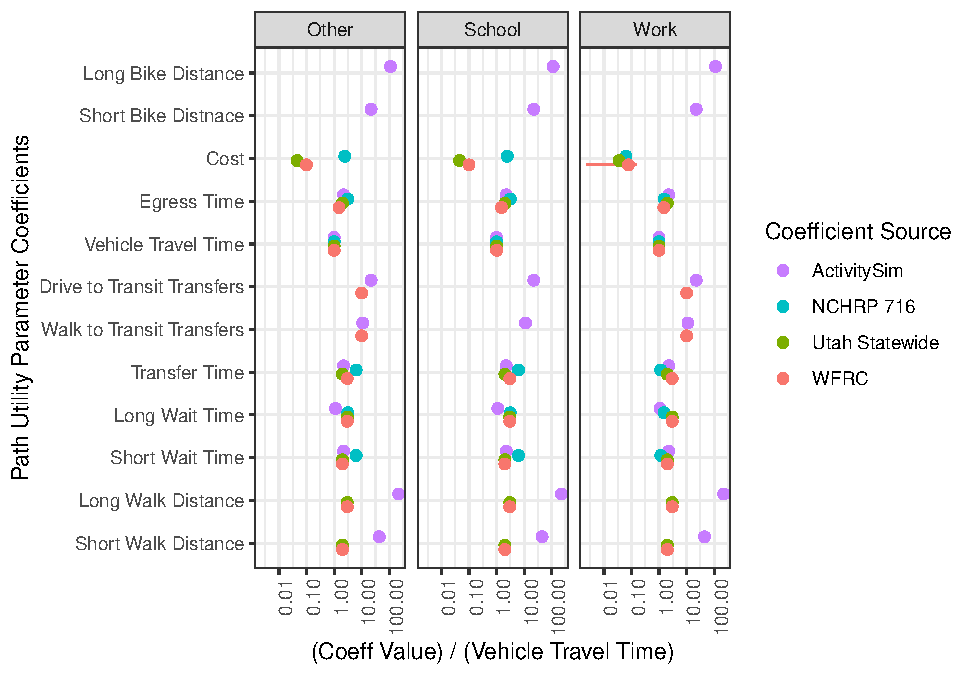
\includegraphics{thesis_files/figure-latex/coef-1} 

}

\caption[Path coefficients model comparison.]{Mode choice path coefficients model comparison by tour purpose.}\label{fig:coef}
\end{figure}

Lastly, after completing the utility parameter validation we calibrated the mode choice utility function's alternative specific constants. The new ASC value \(\alpha'\) was calculated as:

\begin{equation}
  \alpha_{nk}' = \alpha_{nk} + ln(\frac{T_{nk}^{ASIM}}{T_{nk}^{BEAM}}) \label{eq:eqcalib}
\end{equation}
where \(n\) is auto sufficiency, \(k\) is modal alternative, \(\alpha\) is the previous iteration's ASC value, \(T^{ASIM}\) is ActivitySim trip shares, and \(T^{BEAM}\) is BEAM trip shares. We completed the BEAM calibration through an iterative process of updating ASC values using Equation \eqref{eq:eqcalib}. After completing 15 iterations of compounding Equation \eqref{eq:eqcalib} on the ASC values, the BEAM trip values were within a reasonable range to the ActivitySim target shares. Figure \ref{fig:fig-beam-calib} shows the progress of the calibration targets with the final shares after each iteration.

\begin{figure}
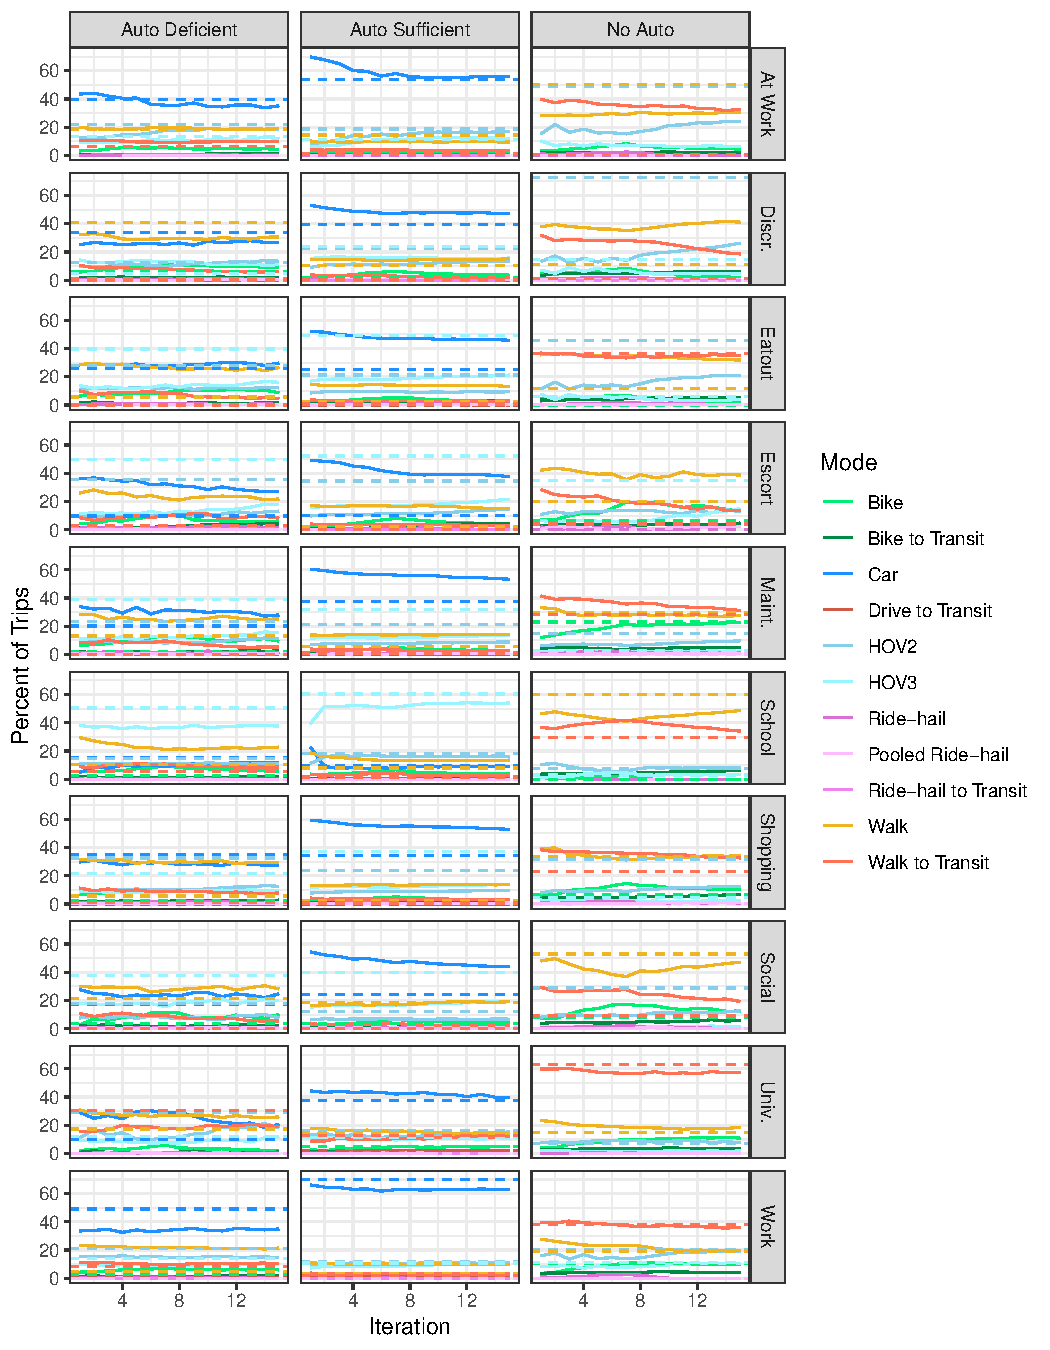
\includegraphics{thesis_files/figure-latex/fig-beam-calib-1} \caption[BEAM mode choice calibration process.]{BEAM mode choice calibration process. Note that the y axis grouping titles are activity types where 'Discr.' represents 'Discretionary' and 'Escort' represents dropping someone off.}\label{fig:fig-beam-calib}
\end{figure}

\hypertarget{meth-scenarios}{%
\section{Case Study Scenarios}\label{meth-scenarios}}

After completing the BEAM validation and BEAM calibration for the case study region, we designed a series of different BEAM experiments. We ran each experiment for a total of 12 iterations using a 15\% population size. More specifically, we conducted nine different experiments, each with a unique ActivitySim-to-BEAM mode choice combination. Table \ref{tab:tbexperiments} provides a short name description of the nine different scenarios.

\begin{table}
\caption[ActivitySim-to-BEAM Mode Choice Combination Names]{ActivitySim-to-BEAM Mode Choice Combination Scenario Names}
\vspace{-10mm}
\renewcommand{\arraystretch}{2}
\[
  \begin{array}{cc|ccc}
    &\multicolumn{1}{c}{} & \multicolumn{2}{c}{\text{ActivitySim}} \\
    && \text{Plans without ride-hail} & \text{Plans with RideHail}\\
    \hline
    & \text{None} & \text{} & \text{AsimRideHail} \\
    \smash{\rotatebox[origin=c]{90}{\text{BEAM}}} & \text{RideHail} & \makecell{\text{BeamRideHail:Path} \\ \text{BeamRideHail:PPL}} & \makecell{\text{AsimBeamRideHail:Path} \\ \text{AsimBeamRideHail:PPL}} \\
    & \text{All} & \makecell{\text{BeamAll:Path} \\ \text{BeamAll:PPL}} & \makecell{\text{AsimBeamAll:Path} \\ \text{AsimBeamAll:PPL}}
  \end{array}
\]
\label{tab:tbexperiments}
\vspace{-5mm}
\end{table}

To better describe the meaning of each scenario in Table \ref{tab:tbexperiments}, we explain the three mode choice descriptors that were altered in each scenario. The first descriptor refers to how ActivitySim's modes were configured, which in Table \ref{tab:tbexperiments} is labeled under \emph{ActivitySim} as \emph{Plans without RideHail} and \emph{Plans with RideHail}. In the naming convention, any name starting with \emph{Asim} refers to any scenario where ride-hailing was included in the input plans from ActivitySim, and any name without \emph{Asim} refers to any a scenario where ride-haling was excluded from the inputs plans from ActivitySim. In other words, the ActivitySim ride-hailing nesting option as shown in Figure \ref{fig:fig-asim-nest} only existed in one version of ActivitySim. Since the daily activity plans generated by ActivitySim were converted to BEAM inputs, this descriptor explains the initial mode choice selections for all trips entered into BEAM.

The second descriptor present in Table \ref{tab:tbexperiments} is labeled under \emph{BEAM} as \emph{None}, \emph{RideHail}, and \emph{All}. These three variables explain which mode choice structure was used in BEAM. These variables also explain which modal alternatives were available for choice within BEAM. The \emph{None} category represents a version of BEAM where all modal innovation was turned off. This means that no mode choice was available and agents did not select to choose alternate modes. The \emph{RideHail} category represented a version of BEAM where modal innovation was partially turned off. All trips that originally took car or carpool modes had modal innovation turned off; their modes were locked. All trips that originally took walk-transit or drive-transit modes, however, were given the option to switch to a ride-haliing mode. Also, all walk modes were given the option to switch to a ride-hail vehicle. \emph{RideHail} represents the version of BEAM where ride-hail and ride-hail transit modes were only given to none-car dependent agents. Finally, the \emph{All} category represents a version of BEAM where modal innovation was turned on, and all modal alternatives were available for choice. This means that within-day replanning as well as across-day replanning was turned on, and agents could change their trip modes to maximize their utility.

Finally, the third descriptor present in Table \ref{tab:tbexperiments} is labeled as either \emph{Path} or \emph{PPL} and explains which utility variables were used to calculate modal utility. The \emph{Path} option represented the version of BEAM that used Equation \eqref{eq:path}, which used only path type utility parameters to calculate mode choice utility. The \emph{PPL} option represented the version of BEAM that used Equation \eqref{eq:all}, which used all path, person, and location type utility parameters to calculate mode choice utility.

\hypertarget{summary-1}{%
\section{Summary}\label{summary-1}}

Overall, we ran nine different scenarios each with a slightly different ActivitySim-to-BEAM mode choice combination. Each scenario is built from which modes were included in the input plans, which modal alternatives were available for choice, and which utility parameter types were used to calculate the mode choice utility. By altering these three different mode choice characteristics, we hope to better understand the affect different linked activity-based model and multi-agent simulation combinations have on ride-hailing ridership and level of service.

\hypertarget{results}{%
\chapter{Results}\label{results}}

We estimated ride-hailing ridership and level of service for each of the nine previously mentioned ActivitySim-to-BEAM mode choice combinations. Specifically, we estimated ride-hailing ridership, wait time, and utilization. Alongside each other, these results shed light on how different combinations of an activity-based model and multi-agent simulation perform at estimating ride-haling ridership and level of service. We can see how differing mode choice structures affect the use and performance of ride-hailing modes.

\hypertarget{res-ridership}{%
\section{Ridership}\label{res-ridership}}

Table \ref{tab:ridership} shows the number of forecasted trips for the ride-hail, pooled ride-hail, and ride-hail transit type modes for all nine mode choice combinations. Table \ref{tab:ridership} also includes the number of forecasted trips within the plans with ride-hail created by ActivitySim, before the mode choices were changed by BEAM. Lastly, Table \ref{tab:ridership} provides a total percentage column, showing the total percentage of ride-hailing modes in relation to the overall modal distribution.

\begin{table}

\caption[Ride-hail Ridership by Number of Total Trips]{\label{tab:ridership}Forecasted Ride-hail Trip Ridership by Mode Choice Combination Scenario}
\centering
\fontsize{10}{12}\selectfont
\begin{tabular}[t]{lrrrrr}
\toprule
Scenario Name & Ride-hail & Pooled Ride-hail & Ride-hail to Transit & Total & Total (\%)\\
\midrule
\cellcolor[HTML]{D9D9D9}{\em{ActivitySim - Inputs to BEAM}} & \cellcolor[HTML]{D9D9D9}{\em{2412}} & \cellcolor[HTML]{D9D9D9}{\em{1837}} & \cellcolor[HTML]{D9D9D9}{\em{0}} & \cellcolor[HTML]{D9D9D9}{\em{4249}} & \cellcolor[HTML]{D9D9D9}{\em{0.38}}\\
\addlinespace
\cellcolor[HTML]{FAEBD7}{AsimRideHail} & \cellcolor[HTML]{FAEBD7}{269} & \cellcolor[HTML]{FAEBD7}{31} & \cellcolor[HTML]{FAEBD7}{0} & \cellcolor[HTML]{FAEBD7}{300} & \cellcolor[HTML]{FAEBD7}{0.03}\\
\cellcolor[HTML]{FFB6C1}{BeamRideHail:Path} & \cellcolor[HTML]{FFB6C1}{45001} & \cellcolor[HTML]{FFB6C1}{25014} & \cellcolor[HTML]{FFB6C1}{2943} & \cellcolor[HTML]{FFB6C1}{72958} & \cellcolor[HTML]{FFB6C1}{6.18}\\
\cellcolor[HTML]{FFB6C1}{BeamRideHail:PPL} & \cellcolor[HTML]{FFB6C1}{18907} & \cellcolor[HTML]{FFB6C1}{38935} & \cellcolor[HTML]{FFB6C1}{4621} & \cellcolor[HTML]{FFB6C1}{62463} & \cellcolor[HTML]{FFB6C1}{5.34}\\
\cellcolor[HTML]{FFB6C1}{AsimBeamRideHail:Path} & \cellcolor[HTML]{FFB6C1}{21519} & \cellcolor[HTML]{FFB6C1}{40873} & \cellcolor[HTML]{FFB6C1}{5437} & \cellcolor[HTML]{FFB6C1}{67829} & \cellcolor[HTML]{FFB6C1}{5.75}\\
\cellcolor[HTML]{FFB6C1}{AsimBeamRideHail:PPL} & \cellcolor[HTML]{FFB6C1}{47422} & \cellcolor[HTML]{FFB6C1}{27327} & \cellcolor[HTML]{FFB6C1}{3848} & \cellcolor[HTML]{FFB6C1}{78597} & \cellcolor[HTML]{FFB6C1}{6.60}\\
\cellcolor[HTML]{ADD8E6}{BeamAll:Path} & \cellcolor[HTML]{ADD8E6}{4671} & \cellcolor[HTML]{ADD8E6}{1596} & \cellcolor[HTML]{ADD8E6}{38} & \cellcolor[HTML]{ADD8E6}{6305} & \cellcolor[HTML]{ADD8E6}{0.57}\\
\cellcolor[HTML]{ADD8E6}{BeamAll:PPL} & \cellcolor[HTML]{ADD8E6}{3146} & \cellcolor[HTML]{ADD8E6}{6366} & \cellcolor[HTML]{ADD8E6}{121} & \cellcolor[HTML]{ADD8E6}{9633} & \cellcolor[HTML]{ADD8E6}{0.86}\\
\cellcolor[HTML]{ADD8E6}{AsimBeamAll:Path} & \cellcolor[HTML]{ADD8E6}{3470} & \cellcolor[HTML]{ADD8E6}{4596} & \cellcolor[HTML]{ADD8E6}{90} & \cellcolor[HTML]{ADD8E6}{8156} & \cellcolor[HTML]{ADD8E6}{0.73}\\
\cellcolor[HTML]{ADD8E6}{AsimBeamAll:PPL} & \cellcolor[HTML]{ADD8E6}{3153} & \cellcolor[HTML]{ADD8E6}{6031} & \cellcolor[HTML]{ADD8E6}{156} & \cellcolor[HTML]{ADD8E6}{9340} & \cellcolor[HTML]{ADD8E6}{0.83}\\
\bottomrule
\end{tabular}
\end{table}

By comparing scenarios against each other, we can understand how slight differences in the mode choice model can significantly affect estimated ridership totals. We first compare the ActivitySim scenario with the AsimRideHail scenario. The ActivitySim scenario represents the ride-hailing input plans created by ActivitySim before being inserted into BEAM and the AsimRideHail scenario represents how these ride-hailing input plans change in BEAM while undergoing no new mode choice. Comparing these two scenarios we see the estimated 4,249 ride-hailing trips of ActivitySim diminished to 300 trips within BEAM because the AsimRideHail scenario was unable to recreate the same ride-hailing paths as ActivitySim. Then, comparing the \emph{RideHail} and \emph{All} type scenarios with the AsimRideHail scenario and ActivitySim scenario we see that when BEAM mode choice innovation is turned on for all or part of the agents, BEAM predicts significantly higher ridership totals. As a result, we suppose that BEAM is prone to estimating higher ridership totals for ride-hailing modes than ActivitySim when modal innovation is turned on, and lower totals when turned off.

Next, we examine the effect the existence of ride-hailing in the input plans has on ridership. As shown in Table \ref{tab:ridership}, minimal differences in ridership is produced between scenarios with the \emph{Asim} prefix vs.~without. For example, between the BeamRideHail:Path and AsimBeamRideHail:Path scenarios we see that input plans without ride-hail produce 72,958 estimated trips (6.18\%), whereas input plans with ride-hail produce 67,829 estimated trips (5.75\%). Similarly, the gap between the ride-hailing trips of the BeamRideHail:PPL and AsimBeamRideHail:PPL scenario is relatively close, at 62,463 and 78,597 trips (5.34\% and 6.60\%) respectively. Although thousands of trips separate the comparing scenarios, in both cases, less than a 1.5\% difference in total modal distribution occurs. In addition, the output ridership trips are almost identical between the BeamAll:PPL and AsimBeamAll:PPL scenarios and close between the BeamAll:Path and AsimBeamAll:Path scenarios (between 0.50\% and 0.75\% of the total modal distribution). Overall, we see similar ridership results among similar mode choice structures independent of the inclusion of ride-hailing in input plans.

We also notice that different BEAM mode choice models predict different forecasted ride-hailing ridership levels. The \emph{None} type scenario (AsimRideHail) assigns few agents to the ride-hail mode. The \emph{RideHail} type scenarios produce the largest number of ride-hail modes among BEAM mode choice structures. The \emph{All} type scenarios produce more ride-hail modes than the \emph{None} type, but less ride-hail modes than the \emph{RideHail} type. In addition, the \emph{All} type scenarios predicts similar ridership values as ActivitySim. The number of ride-hail only type trips is 2,259 more in the BeamAll:Path scenario than in the ActivitySim scenario. All the \emph{All} type scenarios as well as ActivitySim predict under 1\% total ride-hailing modes. Overall, forecasted ridership is affected significantly by which mode choice structure is used by BEAM; this conclusion is clear.

Finally, we analyze the effect the BEAM utility variables have on forecasted ride-hail ridership totals. Comparing the BeamRideHail:Path and BeamRideHail:PPL scenarios we see ride-hail only ridership decreases (45,001 and 18,907) when using path, person, and location variables, but increases with pooled ride-hail (25,014 and 38,935) and ride-hail transit (2,943 and 4,621). This same pattern occurs when analyzing the difference between the BeamAll:Path and BeamAll:PPL, and AsimBeamAll:Path and AsimBeamAll:PPL scenarios. For some oddity though, AsimBeamRideHail:Path and AsimBeamRideHail:PPL follow an opposite pattern. We acknowledge that not all scenarios follow the same pattern, but hypothesize that in general, using only path variables to estimate ride-hail ridership will result in less total ride-hail ridership than if using all path, person, and location type variables.

\hypertarget{res-waits}{%
\section{Wait Times}\label{res-waits}}

Figure \ref{fig:waits} shows a detailed distribution of wait times for ride-hailing vehicles for the scenarios. As with ridership, we compare the scenarios with the \emph{Asim} prefix against the scenarios without, and see only a slight difference in maximum wait times. Scenarios AsimBeamRideHail:PPL, AsimBeamAll:Path, and AsimBeamAll:PPL have almost identical mean wait times when compared to their counterparts in BeamRideHail:PPL, BeamAll:Path, BeamAll:PPL. We suppose that the existence of ride-hail in the initial plans will not affect \emph{most} ride-hail wait times.

\begin{figure}

{\centering 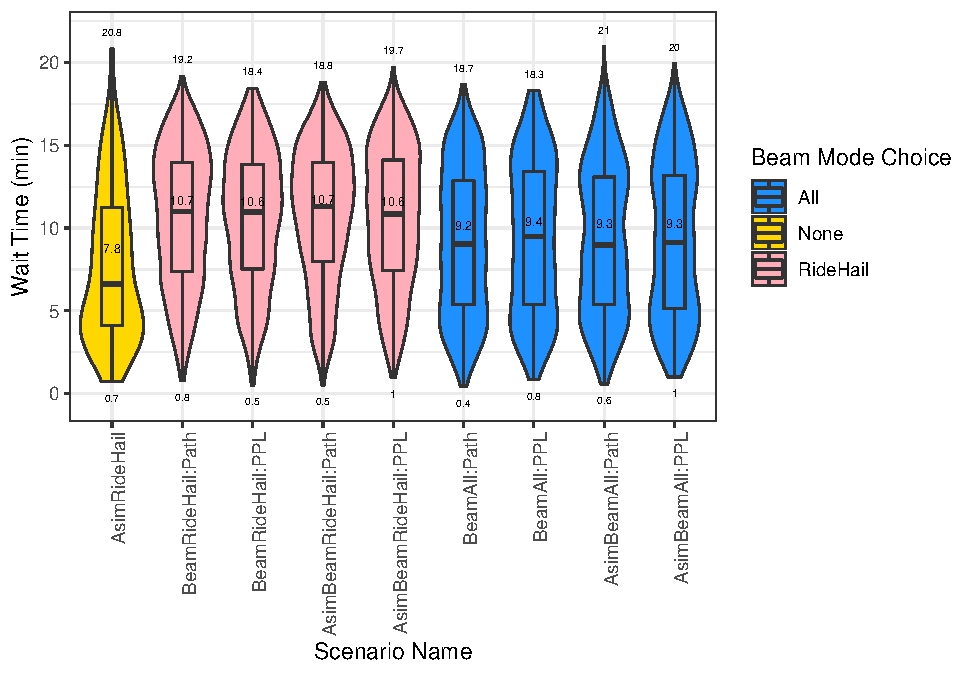
\includegraphics{thesis_files/figure-latex/waits-1} 

}

\caption[Distribution of ride-hail wait times.]{Distribution of ride-hail wait times by mode choice combination scenario.}\label{fig:waits}
\end{figure}

Alternately, comparing different BEAM mode options does significantly affect ride-hail wait times. The \emph{None} type scenario (AsimRideHail) has the largest spread of wait times, the lowest mean wait time, and is ``bottom heavy'' -- referring to the fact that a major cluster of users wait less than 7.5 minutes. The \emph{All} type scenarios have higher mean wait times (\textasciitilde9.3 minutes) than the \emph{None} type and lower mean wait times than the \emph{RideHail} type. Neither top nor bottom heavy, the \emph{All} type scenarios have a more even spread in wait times, ranging from 0.4 to 21 minutes. BEAM seems to paint ride-hail alternatives as more desirable than ActivitySim, as more users are willing to wait longer (12 to 18 minutes in the \emph{All} scenarios). This is especially true with the \emph{RideHail} type scenarios, as a large cluster of users are willing to wait 7.5 to 20 minutes. The \emph{RideHail} type scenarios have the largest mean wait times (\textasciitilde10.65 minutes). By simply viewing the wait time distribution, we see a difference in level of service depending on model structure. Wait time is significantly affected by which mode choice structure is used by BEAM, just like as was concluded with ridership.

We also conducted a statistical comparison between quantile ranges between all three model structures. Using a quantile test based on the method proposed in Wilcox et al. (2014), a significant statistical difference exists between the None and All models, the All and RideHail models, and the None and RideHail models at the 20th and 50th percentile levels. At the 80th percentile level, a significant difference exists between the All and RideHail models and the None and RideHail models, but not between the None and All models. The results of these statistical tests prove that a different level of service will result based on which mode choice model structure is used.

The last group to compare collectively is between the Path and PPL models. By comparing BeamRideHail:Path and BeamRideHail:PPL, BeamAll:Path and BeamAll:PPL, and AsimBeamAll:Path and AsimBeamAll:PPL, we see that the Path models estimate a slightly higher maximum wait time. In addition, BeamRideHail:Path and AsimBeamRideHail:Path seem to have a larger cluster above a 10 minute wait time than BeamRideHail:PPL and AsimBeamRideHail:PPL. Besides these two observations though, the differences between utility parameters is minimal. Although ridership was affected by which utility parameters were used, wait time is only slightly affected.

Overall, by analyzing the ridership and wait times among different mode choice structures we learn that ride-hailing ridership and level of service is significantly affected by which mode choice structure is used in BEAM. The mode choice model structure one uses to estimate ride-hailing level of service and wait time matters! We also suggest that initial plans, and whether or not they include ride-hail, do not significantly affect the level at which BEAM estimates ridership or wait times. Lastly, we hypothesize that using all path, person, and location type variables will increase total ridership. We also suggest that the lack of person attributes in the utility equation may cause pooled and transit ride-hail options to look less appealing. Section \ref{deep-look} takes a deeper look at why some of these patterns in the ridership and wait times results exist.

\hypertarget{deep-look}{%
\section{Mode Choice Structures}\label{deep-look}}

The results from Table \ref{tab:tbexperiments} and the results from Figure \ref{fig:waits} can be explained further by understanding the original setup of the experiments. The clearest distinction in ridership and wait times exist between BEAM mode choice structures. The \emph{None}, \emph{RideHail}, and \emph{All} structure types each produce results at different magnitudes, drawing on the conclusion that mode choice model structure matters. Therefore, to best understand these structures, we explore their inner-workings.

\hypertarget{type1}{%
\subsection{None Mode Choice Model}\label{type1}}

The \emph{None} mode choice model produces the lowest ridership and shortest wait time values. With modal innovation turned off, this model did not allow agents to choose new modes, and averted them to walk modes if their current trip mode was deemed ``impossible''. This is verified by looking at Table \ref{tab:noneloss}. Iteration 0 (start) shows the number of ride-hailing modes input to BEAM. By the end of iteration 0, however, more than half the initial ride-hailing selections estimated by ActivitySim were lost. Then, by the end of the final iteration, only 300 ride-hailing trips remained. At the same time, total walk modes increased across each iteration. BEAM was unable to match agents with most of ActivitySim's ride-hailing predictions.

\begin{table}

\caption{\label{tab:noneloss}Loss of Ride-hailing Trips in the None Mode Choice Model}
\centering
\resizebox{\linewidth}{!}{
\begin{tabular}[t]{lllll}
\toprule
Iteration & Ride-hail & Pooled Ride-hail & Ride-hail Transit & Total\\
\midrule
0 (start) & 2412 & 1837 & 0 & 4249\\
0 (end) & 978 & 615 & 0 & 1593\\
12 (end) & 269 & 21 & 0 & 300\\
\bottomrule
\end{tabular}}
\end{table}

\hypertarget{type3}{%
\subsection{All Mode Choice Model}\label{type3}}

The \emph{All} BEAM mode choice model uses the same mode choice utility function as ActivitySim and has all modal alternatives available. This adjusted model structure helps us understand why we obtained much higher ridership than with the \emph{None} Model. Figure \ref{fig:piechart} shows from which modes the model assigned agents who switched to ride-hailing came from; in other words, its a comparison of the the trips with ride-hailing after the final iteration and their original modes in the input plans. Interestingly enough, the \emph{All} model assigns the majority of agents who select ride-hail to a car type mode. We define car type modes as either a car, a high occupancy vehicle with two passengers (HOV2), or a high occupancy vehicle with three or more passengers (HOV3)

\begin{figure}

{\centering 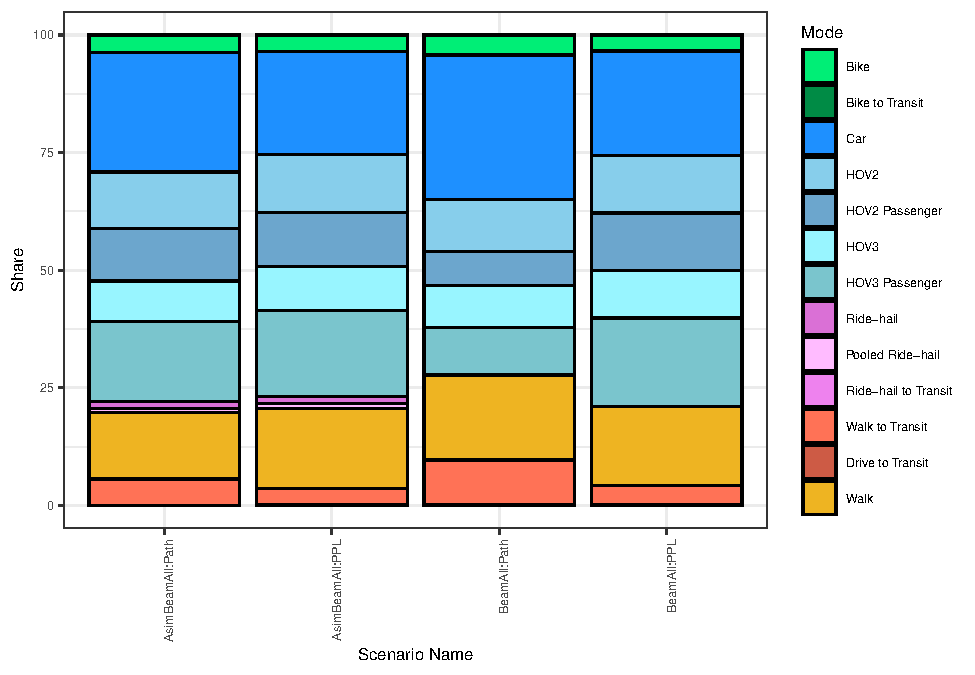
\includegraphics{thesis_files/figure-latex/piechart-1} 

}

\caption[Original mode choices of agents who were assigned to ride-hail.]{Original mode choices of agents who were assigned to a ride-hail type mode.}\label{fig:piechart}
\end{figure}

We offer some factors as to why the \emph{All} model assigns so many car users to ride-hailing modes. The first is the array of utility parameters boosted the ride-hailing utility, making ride-hailing options attractive alternatives. Figure \ref{fig:sankey} provides sufficient evidence for this claim. Figure \ref{fig:sankey} shows a Sankey diagram of all modal decisions at the start of each iteration for those agents in the AsimBeamAll:PPL scenario who the model assigned the ride-hail mode by the end of the 12th iteration. In other words, it shows from what modes the final ride-hail modes came from. For example, of the approximate 6,000 trips with a ride-hail mode assigned after iteration 12, on those same trips in iteration 1 more than 2,000 of them began as car trips, in iteration 5 about 2,000 of them began as car trips, and in iteration 11 less than 1,000 of them began as car trips. Similar logic can be applied to other iterations and to other modes. In the figure's key, the mode ``Cleared Mode'' describes those modes that were cleared and reset at the beginning of each iteration. Notice how many of the Car, HOV2, HOV2 Passenger, HOV3, and HOV3 Passenger modes shift into the ``Cleared Mode'' category each iteration. Also notice in the subsequent iteration how many of those ``Cleared Mode'' choices shift to ride-hailing modes. A shift from the ``Cleared Mode'' choice to ride-hail represents those agents from whom the model assigned a mode based on the utility value.

\begin{sidewaysfigure}

\centering
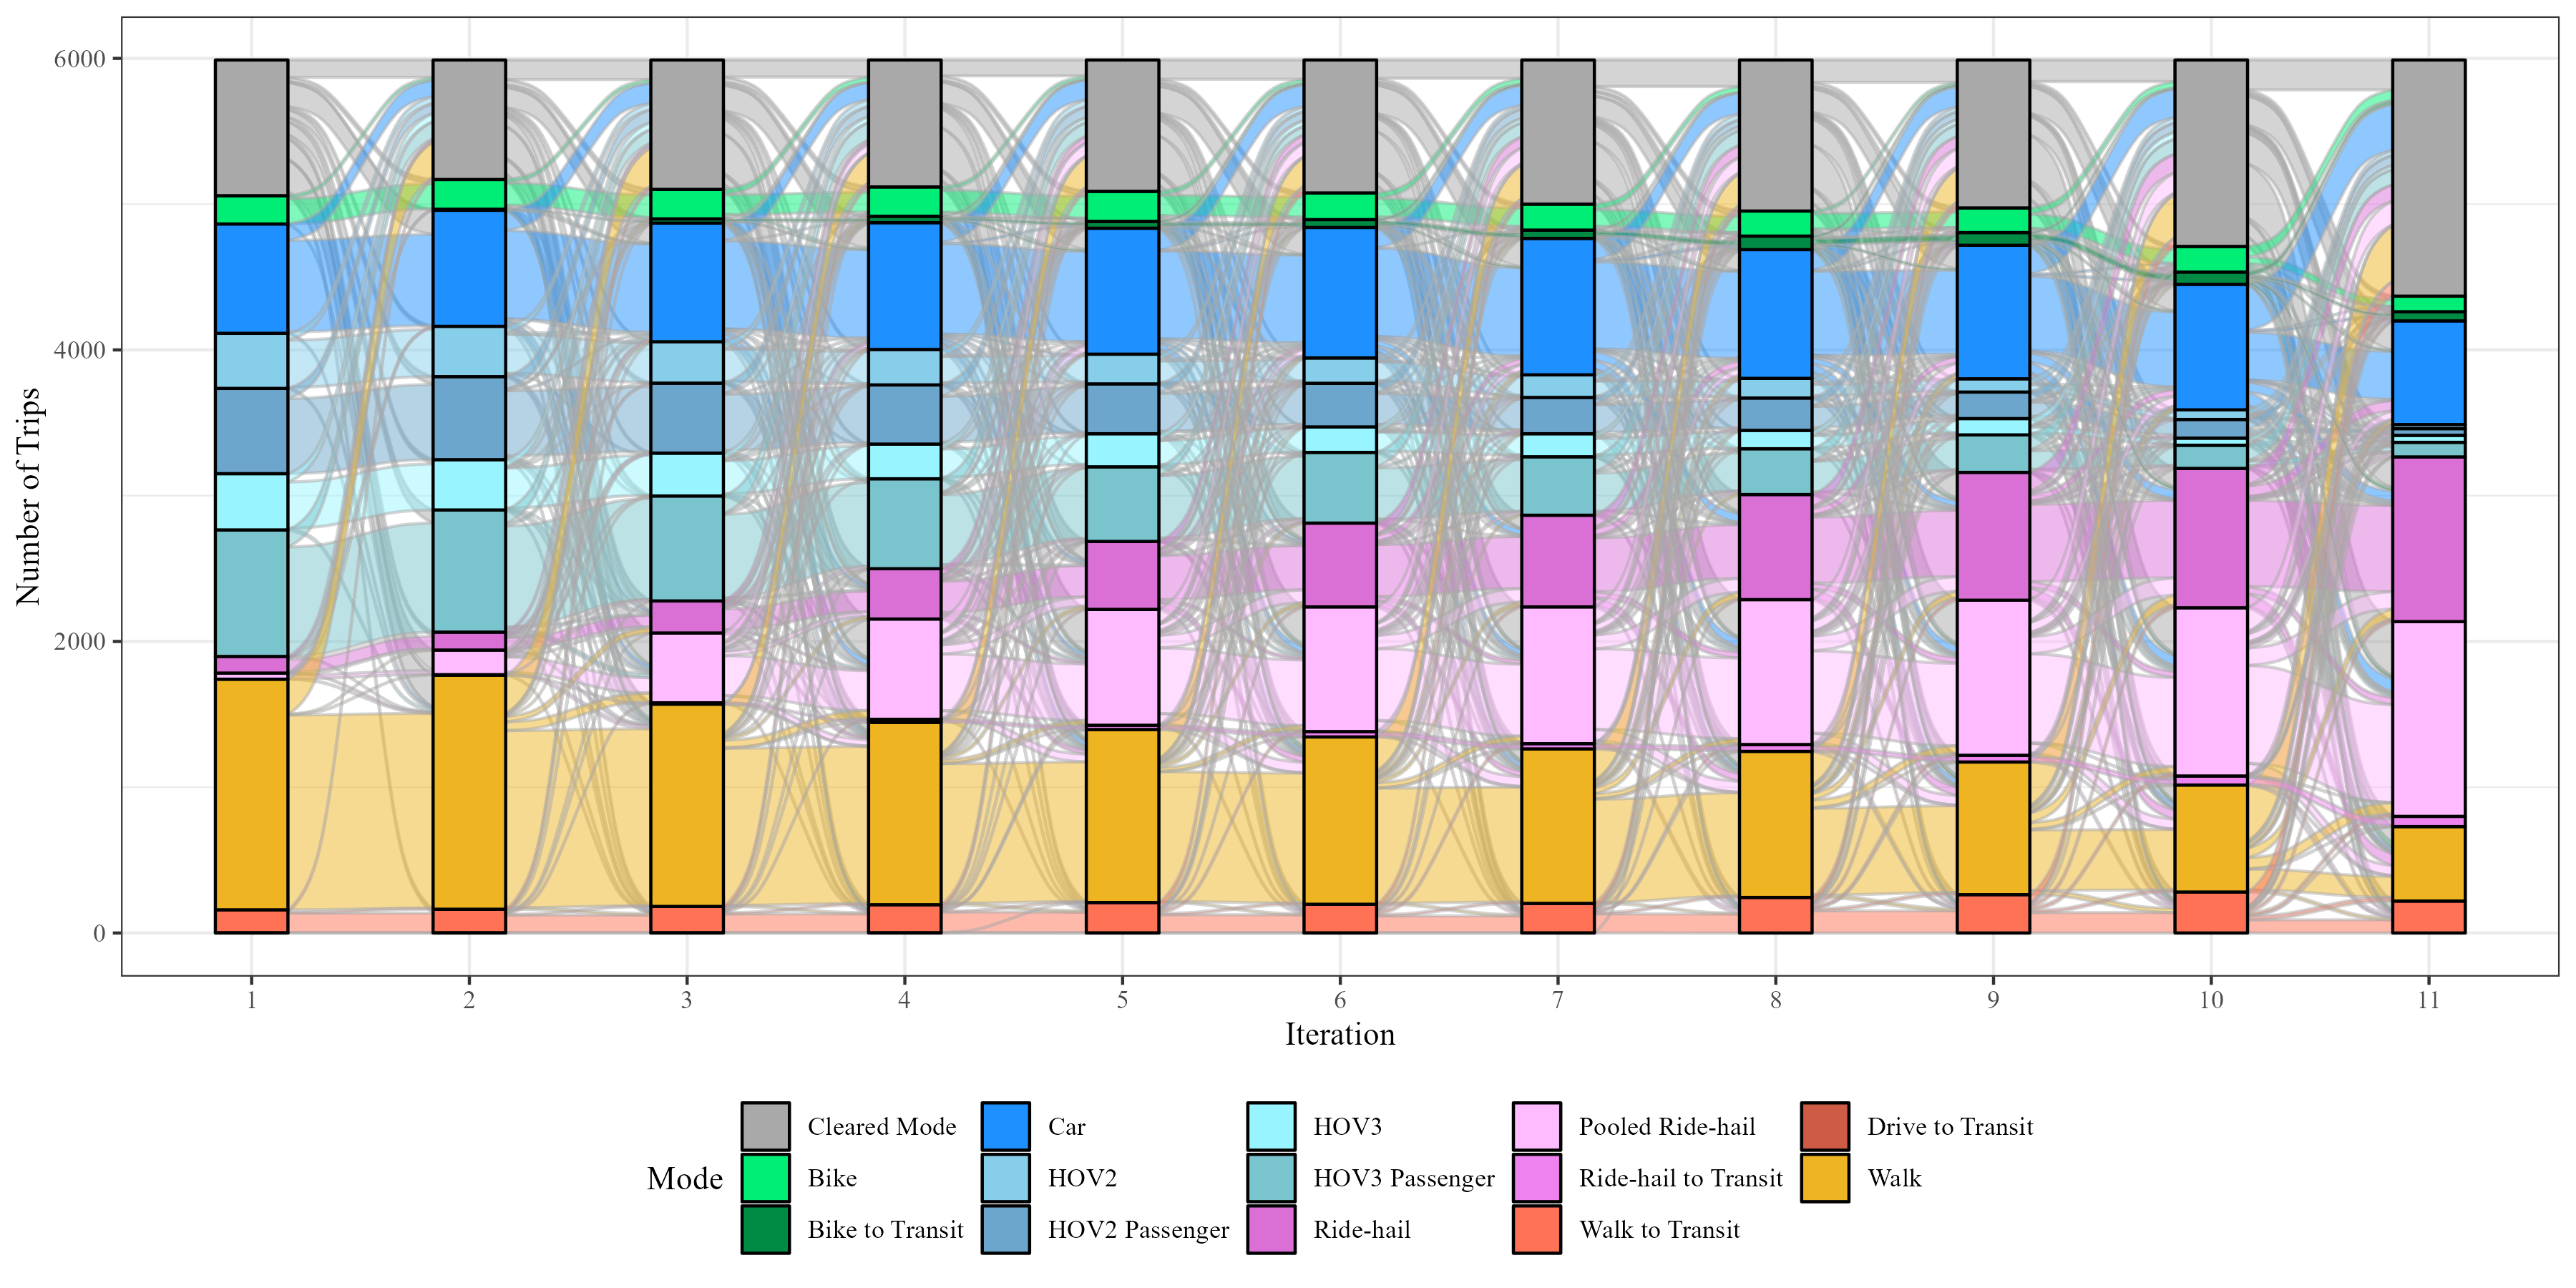
\includegraphics[width = 1.05\paperwidth]{planshifts.png}
\caption[Selection process of agents who the model assigned to ride-hail.]{The modal selections at each iteration start of those agents who were assigned a ride-hailing mode at the end of iteration 12 (AsimBeamAll:PPL Scenario).}
\label{fig:sankey}

\end{sidewaysfigure}

Figure \ref{fig:sankey2} further proves that the \emph{All} model assigns many agents to use ride-hailing modes because the utility parameters represent them as attractive alternatives. Figure \ref{fig:sankey2} displays the total number of ride-hailing trips at the end of each iteration as well as which modes were used on those same trips at the beginning of the iteration for the AsimBeamAll:PPL scenario. Notice how for the majority of iterations, a substantial share of agents are assigned from the ``Cleared Mode'' category to a ride-hailing category instead. Looking closer at this figure also leads us to believe that many ride-hailing trips are not held constant across each iteration. In other words, many ride-hailing trips at the end of one iteration are not the same ride-hailing trips at the end of the next iteration. Although the number of total ride-hailing increases slightly across each iteration, the model assigns a large portion of new individuals to use ride-hail each iteration. This suggests that the model may not be learning which users are ``best'' for ride-hailing, at least not within only 12 iterations.

\begin{sidewaysfigure}

\centering
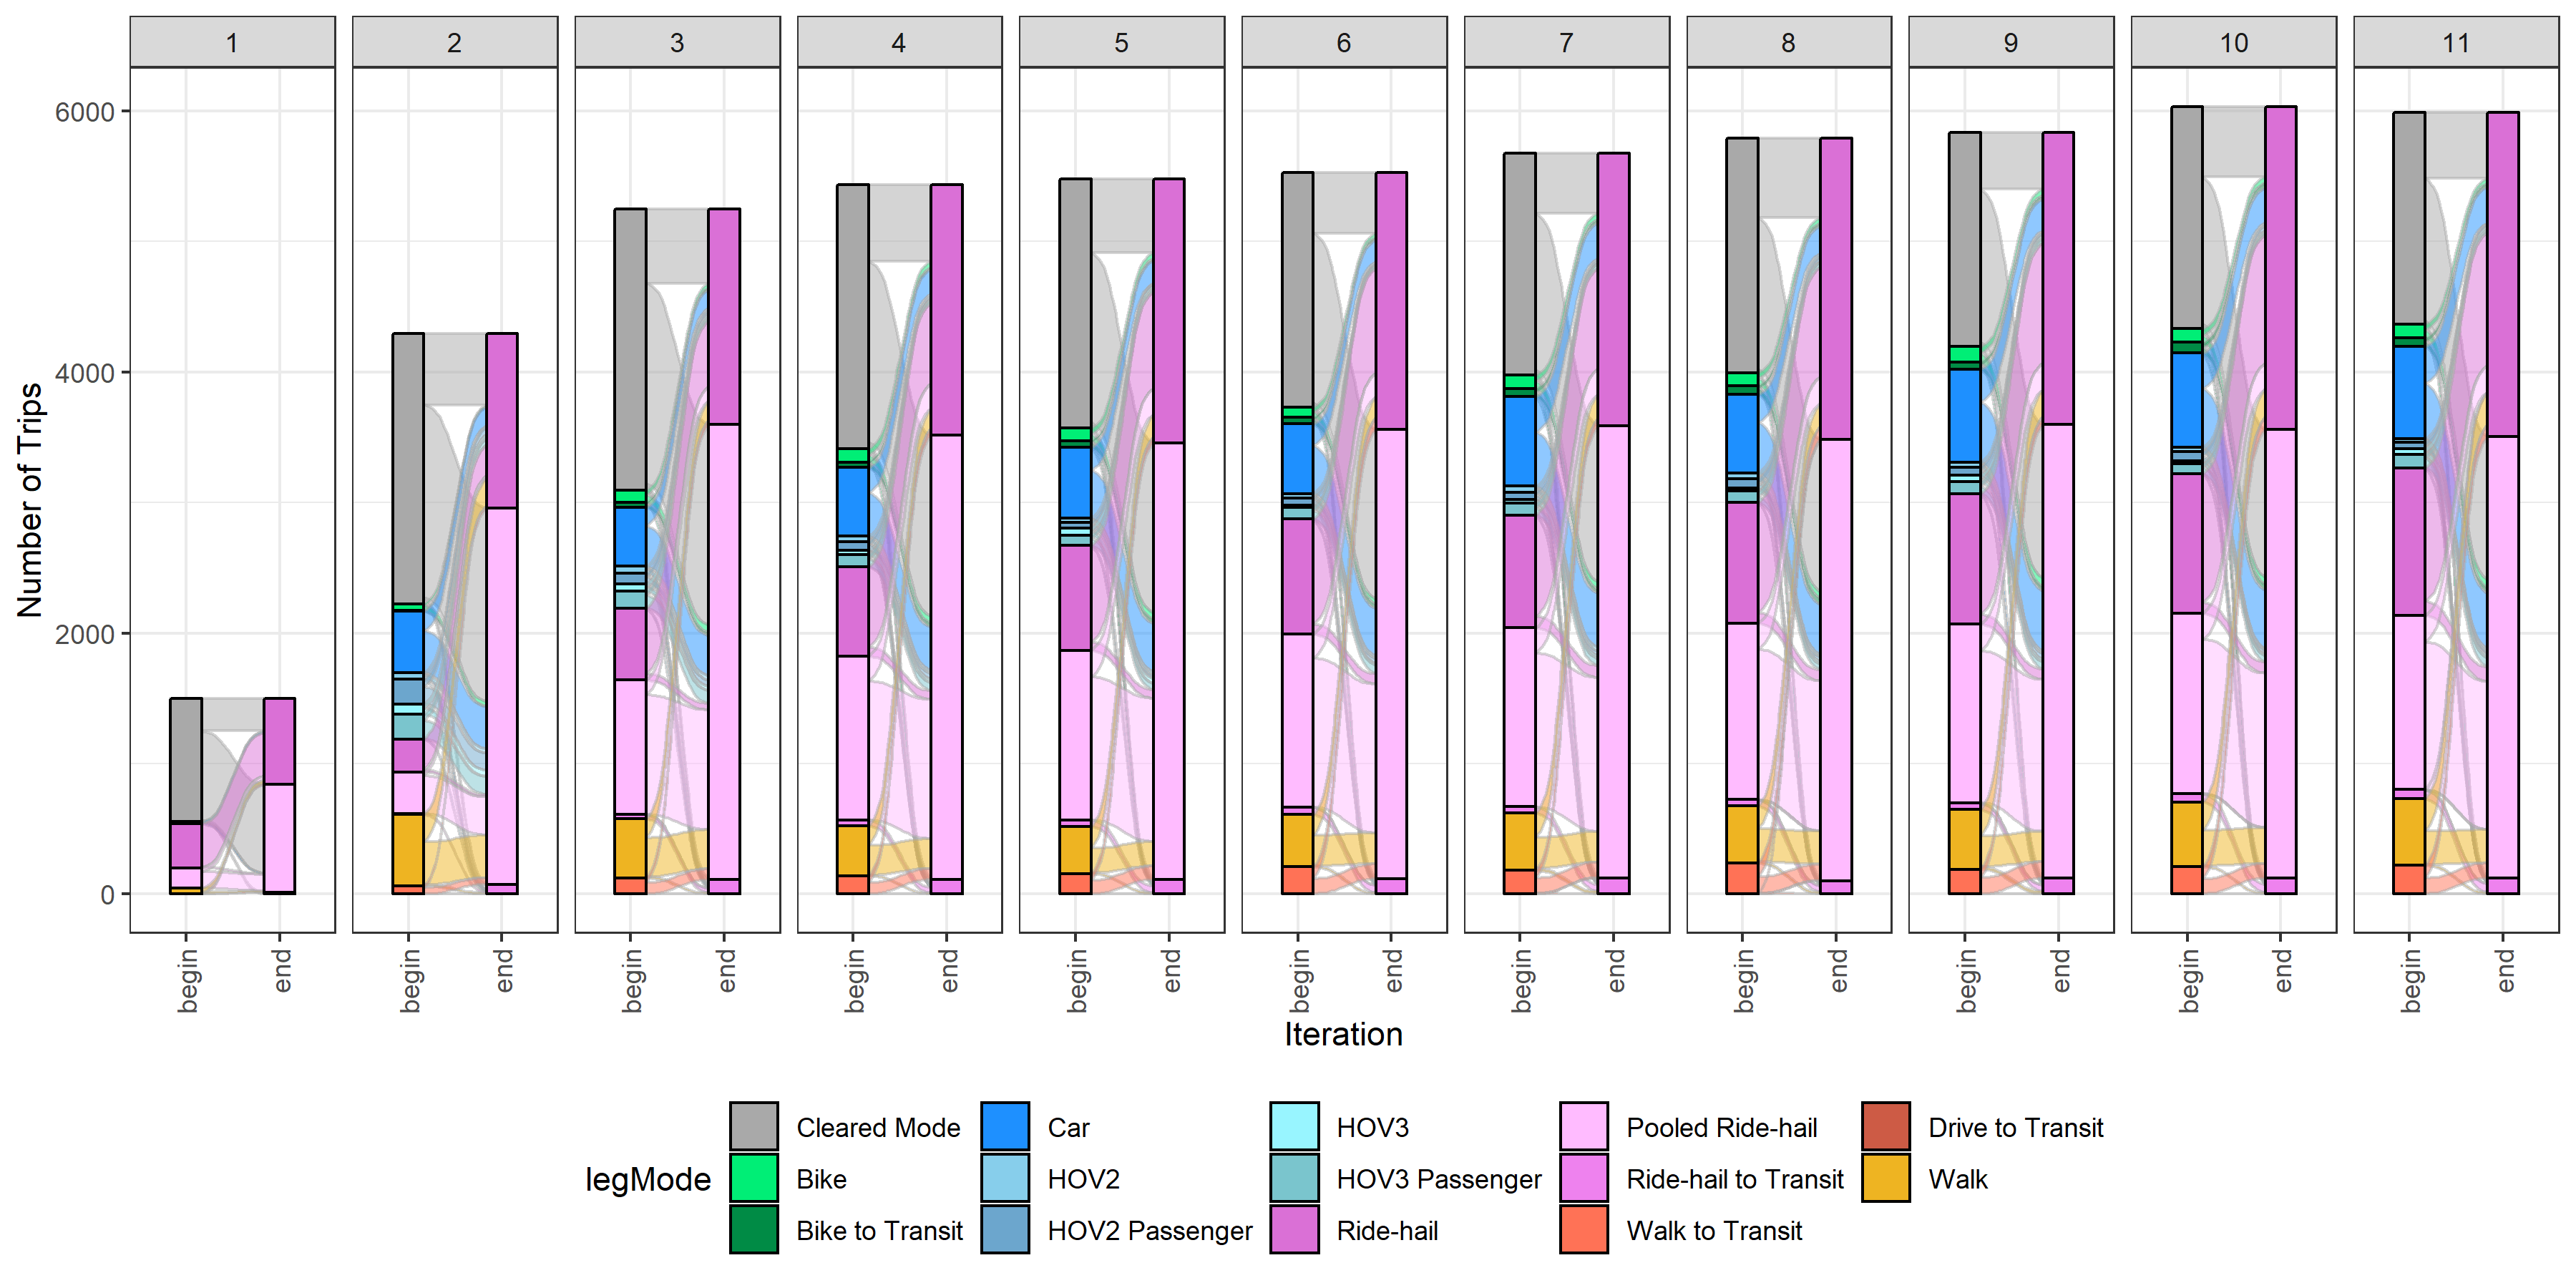
\includegraphics[width = 1.05\paperwidth]{planshifts_facet.png}
\caption[Trips that switch to ride-hail by iteration.]{The modal selections at each iteration start of the agents who were assigned a ride-hailing mode at each corresponding iteration end (AsimBeamAll:PPL Scenario).}
\label{fig:sankey2}

\end{sidewaysfigure}

The last deduction from Figure \ref{fig:sankey2} that we make is from the portion of trips that originate from car and walk trips. The \emph{All} model is changing car and walk type trips directly into ride-hailing trips without first entering them into the ``Cleared Mode'' stage. Although we do not fully understand why this occurs, we do have a few hypotheses. One suggestion is that a slight error may exist in the internal mode choice program structure that may have allowed some car and walking trips to undergo mode choice even when they were not supposed to. Another hypothesis is that BEAM's trip based mode choice structure forced some car users to switch modes when a car pathway was not deemed feasible. If this occurred, BEAM's complex car tracking algorithm would have left the car at the previous location, making it unusable on future trips. In other words, the model would have ``lost'' the agent's car. Overall, the increase in ridership in the \emph{All} model can be explained by ride-hailing being an attractive alternative along with a possible error with the internal mode choice structure or the building of feasible car routes.

\hypertarget{type2}{%
\subsection{Ridehail Mode Choice Model}\label{type2}}

Finally, the way the \emph{RideHail} BEAM mode choice model was constructed explains why ridership and wait times were high. The \emph{RideHail} model only allowed the assignment of walk and transit users to ride-hailing modes; car-type modes remained locked across each iteration. Whenever a ride-hailing path could be built, the \emph{RideHail} model automatically provided all walk modes the option to choose ride-hail or ride-hail pooled and all transit modes the option to choose ride-hail transit. Although it made logical sense to lock all car-type modes (for reasons described in Section \ref{type3}), by providing ride-hail options only to walk and transit users, ridership increased even more than in the \emph{All} scenario. The increase in ridership occurred because 1) BEAM's adjusted code forced ride-hail to be an option in almost all cases, and 2) in most cases ride-hail was calculated to be more attractive than walk or transit modes.

Table \ref{tab:timeutil} provides evidence in ride-hail being an attractive mode choice alternative. Table \ref{tab:timeutil} displays the ride-hail time utilization for each of the scenarios performed. The same ride-hail fleet was used in each of the nine scenario, composed of 952 ride-hailing driver shifts. Ride-hail time utilization was calculated as the sum of all the driver shift times divided by the sum of all passenger occupied ride-hailing travel time. The AsimRideHail scenario had the lowest ride-hail time utilization, at only 4.0\%. Interestingly, the \emph{All} type scenarios ranged from 53.1\% to 62.5\% ride-hail time utilization. This explains the higher wait times shown in Figure \ref{fig:waits}. Finally, by analyzing the ride-hail time utilization for the \emph{RideHail} scenarios, we fully understand how attractive ride-hail was. With 70.3\% to 73.8\% of ride-hail time utilization present for the \emph{RideHail} scenarios, we see three fourths of each driver's shift was used to transport passengers. This explains the attractiveness of the choice, the extreme increase in ridership, and also the increased wait time for the \emph{RideHail} type scenarios. Lastly, Table \ref{tab:timeutil} provides evidence that ride-hailing ridership and wait times are a function of model structures, as the only meaningful difference in utilization exists between model structures.

\begin{table}

\caption[Percent Ride-hail Time Utilization]{\label{tab:timeutil}Percent Ride-hail Time Utilization by Mode Choice Combination Scenario}
\centering
\begin{tabular}[t]{lr}
\toprule
Scenario Name & Ride-hail Time Utilization\\
\midrule
AsimRideHail & 4.0\\
BeamRideHail:Path & 73.8\\
BeamRideHail:PPL & 70.3\\
AsimBeamRideHail:Path & 71.4\\
AsimBeamRideHail:PPL & 72.6\\
\addlinespace
BeamAll:Path & 62.5\\
BeamAll:PPL & 53.1\\
AsimBeamAll:Path & 58.7\\
AsimBeamAll:PPL & 53.1\\
\bottomrule
\end{tabular}
\end{table}

\hypertarget{summary-2}{%
\section{Summary}\label{summary-2}}

As seen by the explanation of the structure of the \emph{None}, \emph{All}, and \emph{RideHail} type scenarios, how BEAM's different mode choice structures were programmed affected ride-hailing ridership and wait time. Fortunately, Section \ref{discussion} describes the deeper meaning behind the effect different mode choice structure have on ride-hailing ridership and level of service forecasts.

\hypertarget{discussion}{%
\chapter{Discussion and Conclusion}\label{discussion}}

The results presented in Section \ref{results} show that mode choice structure significantly affects forecasts of ride-hailing ridership and service capabilities. Slight changes to which mode choice alternatives are available in the multi-agent simulation as well as which mode choice utility function is used impacts ridership and level of service greatly. In addition, the programming of the internal multi-agent simulation choice structure has a huge effect on results. When pairing together an activity-based model and a multi-agent simulation in efforts to forecast ride-hailing capabilities, the way the linked mode choice model is setup matters significantly. Although we did not conclude which model structure is most accurate in this research, we suggest to explore this idea in further research.

In addition to learning the effect mode choice model has on estimating ride-hailing ridership and level of service, we found that when modal innovation was turned on, the BEAM mode choice structures had a tendency to overstate demand when compared to ActivitySim. The results also suggest that whether or not ride-hailing exists in the multi-agent simulation's input plans does not make a significant difference to ride-hailing ridership or wait time forecasts. If the multi-agent simulation deemed a ride-hailing path as unfeasible, those agents would be reassigned a different mode.

\hypertarget{further-research}{%
\section{Further Research}\label{further-research}}

The results suggest that the primary area of further research remain at discovering which mode choice model structure estimate accurate ridership and level of service forecasts. In this research we concluded that mode choice model structure matters, but were unable to determine which among those options matches most closely to regional totals. A second area of further research could be to balance the ridership and level of service estimates between an activity-based model and multi-agent simulation using a feedback loop. We suggest an iterative process where the ride-hailing travel and wait times of the multi-agent simulation are inputted back into the activity-based model and the recalculated activity-based model ridership and usage values are inputted back into the multi-agent simulation. This process would continue, working off of each other, until the desired equilibrium and optimization of the ride-hailing system is achieved. By better aligning the two models, this iterative process could establish realistic and reliable ride-hailing ridership and level of service forecasts.

\hypertarget{limitations}{%
\section{Limitations}\label{limitations}}

Various components of the multi-agent simulation, BEAM, were not perfected. First, the mode choice coefficients in BEAM were not calibrated to exact regional values, and did not represent a completely accurate total modal distribution. In addition, some limitations existed within the BEAM software because BEAM was in development throughout the life of this project. One example is that activity plans remained constant across each iteration. Similarly, BEAM is not a tour based model whereas ActivitySim is. The mode choice models we developed within BEAM also included a few limitations. The \emph{All} structure had various car-matching difficulties as well as path-building difficulties. The \emph{RideHail} structure gave the ride-hail alternative to all individuals instead of only those who had undergone across day replanning.

The two biggest limitations with the input files related to the driver fleet and the network file. The driver fleet did not factor in university and school location when statistically modeling the start location of each ride-hail vehicle. Second, the network file we used only included main roadways, because it was too difficult to develop a reliable all streets network from the resources available. The last significant limitation of the research was that the results were from the 12th iteration of a 15\% scenario size. Due to our limited resources with computing power, larger scenarios with more iterations was too computationally heavy for our computers.

\hypertarget{conclusion}{%
\section{Conclusion}\label{conclusion}}

The increasing usage of on-demand transport modes such as ride-hailing and microtransit has challenged forecasters with finding the best methodology to capturing behavior related to these new modes. Spatial analysis, activity-based models, and multi-agent simulation are common methodological approaches, but some professional disagreement exists as to which approach is best for forecasting the availability and service capabilities of on-demand services. Additional question surrounds how successful a paired activity-based model and multi-agent simulation would fare in practice. By using the daily activity plans generated by ActivitySim, an activity-based model, as inputs to BEAM, a multi-agent simulation tool, we constructed nine different model combinations where the choice of ride-hailing varied between ActivitySim and BEAM. We also adjusted the mode choice utility equation between each model combination. By analyzing the ride-hailing ridership and level of service between each methodological combination, we found that how one pairs an activity-based model and multi-agent simulation greatly affects the ride-hailing ridership and level of service estimates. Linking together an activity-based model and multi-agent simulation is a promising approach to forecasting the performance of ride-hailing services, however, further research is required to 1) understand which combination is best and to 2) better synchronize the estimates between the two models.

Overall, accurately predicting the behavior and service capabilities of on-demand services is the key to a sustainable future. Ride-hailing and other novel modes are central to clean air, organized cities, and the effective movement of people. By accurately predicting the usage of ride-hailing and microtransit vehicles, we can help improve our cities and our lives. Overall, we can directly change the course of our future by how we estimate ride-hailing and other travel behavior, and so, should we not estimate it with the best approaches available? By understanding the power different model structures can have in estimating ride-haling services, this research along with corresponding future research are the stepping stones in the mission to accurately predict the ever changing behavior and capabilities of transportation itself.

\hypertarget{references}{%
\chapter*{References}\label{references}}
\addcontentsline{toc}{chapter}{References}

\hypertarget{refs}{}
\begin{CSLReferences}{1}{0}
\leavevmode\vadjust pre{\hypertarget{ref-rsg21}{}}%
ActivitySim. (2021). An advanced activity-based travel demand model built by and for users. In \emph{RSG}. \href{https://rsginc.com/activitysim-\%20white-paper/\#advanced-activity-based-travel-demand-model}{https://rsginc.com/activitysim- white-paper/\#advanced-activity-based-travel-demand-model}

\leavevmode\vadjust pre{\hypertarget{ref-agrc}{}}%
AGRC. (2021). \emph{Automated geographic reference center}. \url{https://gis.utah.gov/}

\leavevmode\vadjust pre{\hypertarget{ref-amblard15}{}}%
Amblard, F., Daudé, E., Gaudou, B., Grignard, A., Hutzler, G., Lang, C., Marilleau, N., Nicod, J.-M., Sheeren, D., \& Taillandier, P. (2015). Introduction to NetLogo. In \emph{Agent-based spatial simulation with netlogo} (pp. 75--123). Elsevier.

\leavevmode\vadjust pre{\hypertarget{ref-bazghandi12}{}}%
Bazghandi, A. (2012). Techniques, advantages and problems of agent based modeling for traffic simulation. \emph{International Journal of Computer Science Issues (IJCSI)}, \emph{9}(1), 115.

\leavevmode\vadjust pre{\hypertarget{ref-beam}{}}%
BEAM. (2022). \emph{Behavior, energy, autonomy, and mobility}. Lawrence Berkeley National Laboratory the UC Berkeley Institute for Transportation Studies. \url{https://beam.readthedocs.io/en/develop/users.html}

\leavevmode\vadjust pre{\hypertarget{ref-becker20}{}}%
Becker, H., Balac, M., Ciari, F., \& Axhausen, K. W. (2020). Assessing the welfare impacts of shared mobility and mobility as a service (MaaS). \emph{Transportation Research Part A: Policy and Practice}, \emph{131}, 228--243.

\leavevmode\vadjust pre{\hypertarget{ref-biehl19}{}}%
Biehl, A., Ermagun, A., \& Stathopoulos, A. (2019). Utilizing multi-stage behavior change theory to model the process of bike share adoption. \emph{Transport Policy}, \emph{77}, 30--45.

\leavevmode\vadjust pre{\hypertarget{ref-bowman98}{}}%
Bowman, J. L. (1998). \emph{The day activity schedule approach to travel demand analysis} {[}PhD thesis{]}. Massachusetts Institute of Technology.

\leavevmode\vadjust pre{\hypertarget{ref-nchrp}{}}%
Cambridge Systematics, Inc., Vanasse Hangen Brustlin, Inc., Corporation, G., Bhat, C. R., Shapiro Transportation Consulting, L., \& Martin/Alexiou/Bryson, P. (2012). Travel demand forecasting: Parameters and techniques. In \emph{NCHRP report 716} (pp. 55--60). Transportation Research Board.

\leavevmode\vadjust pre{\hypertarget{ref-chen21}{}}%
Chen, L., Thakuriah, P. V., \& Ampountolas, K. (2021). Short-term prediction of demand for ride-hailing services: A deep learning approach. \emph{Journal of Big Data Analytics in Transportation}, \emph{3}(2), 175--195.

\leavevmode\vadjust pre{\hypertarget{ref-cho22}{}}%
Cho, S.-H., \& Shin, D. (2022). Estimation of route choice behaviors of bike-sharing users as first-and last-mile trips for introduction of mobility-as-a-service (MaaS). \emph{KSCE Journal of Civil Engineering}, 1--12.

\leavevmode\vadjust pre{\hypertarget{ref-ciari16}{}}%
Ciari, F., Balac, M., \& Axhausen, K. W. (2016). Modeling carsharing with the agent-based simulation MATSim: State of the art, applications, and future developments. \emph{Transportation Research Record}, \emph{2564}(1), 14--20.

\leavevmode\vadjust pre{\hypertarget{ref-r5}{}}%
Conveyal. (2022). \emph{R5: Rapid realistic routing on real-world and reimagined networks}. \url{https://github.com/conveyal/r5}

\leavevmode\vadjust pre{\hypertarget{ref-correa17}{}}%
Correa, D., Xie, K., \& Ozbay, K. (2017). Exploring the taxi and uber demand in new york city: An empirical analysis and spatial modeling. \emph{96th Annual Meeting of the Transportation Research Board, Washington, DC}.

\leavevmode\vadjust pre{\hypertarget{ref-dean21}{}}%
Dean, M. D., \& Kockelman, K. M. (2021). Spatial variation in shared ride-hail trip demand and factors contributing to sharing: Lessons from chicago. \emph{Journal of Transport Geography}, \emph{91}, 102944.

\leavevmode\vadjust pre{\hypertarget{ref-dong20}{}}%
Dong, X. (2020). Trade uber for the bus? \emph{Journal of the American Planning Association}, \emph{86}(2), 222--235.

\leavevmode\vadjust pre{\hypertarget{ref-dong18}{}}%
Dong, Y., Wang, S., Li, L., \& Zhang, Z. (2018). An empirical study on travel patterns of internet based ride-sharing. \emph{Transportation Research Part C: Emerging Technologies}, \emph{86}, 1--22.

\leavevmode\vadjust pre{\hypertarget{ref-gomes21}{}}%
Gomes, V. A., Caldas, M., \& Pitombo, C. S. (2021). An investigation of trip-chaining behaviour based on activity participation, socioeconomic variables and aggregated characteristics of modal alternatives. \emph{Revista Transportes}, \emph{29}(1), 21--41.

\leavevmode\vadjust pre{\hypertarget{ref-hasnine21}{}}%
Hasnine, M. S., \& Nurul Habib, K. (2021). Tour-based mode choice modelling as the core of an activity-based travel demand modelling framework: A review of state-of-the-art. \emph{Transport Reviews}, \emph{41}(1), 5--26.

\leavevmode\vadjust pre{\hypertarget{ref-horl19}{}}%
Hörl, S., Balać, M., \& Axhausen, K. W. (2019a). Pairing discrete mode choice models and agent-based transport simulation with MATSim. \emph{2019 TRB Annual Meeting Online}, 19--02409.

\leavevmode\vadjust pre{\hypertarget{ref-horl19b}{}}%
Hörl, S., Ruch, C., Becker, F., Frazzoli, E., \& Axhausen, K. W. (2019b). Fleet operational policies for automated mobility: A simulation assessment for zurich. \emph{Transportation Research Part C: Emerging Technologies}, \emph{102}, 20--31.

\leavevmode\vadjust pre{\hypertarget{ref-hosseinzadeh21}{}}%
Hosseinzadeh, A., Algomaiah, M., Kluger, R., \& Li, Z. (2021). Spatial analysis of shared e-scooter trips. \emph{Journal of Transport Geography}, \emph{92}, 103016.

\leavevmode\vadjust pre{\hypertarget{ref-hyland18}{}}%
Hyland, M., Hong, Z., Farias Pinto, H. K. R. de, \& Chen, Y. (2018). Hybrid cluster-regression approach to model bikeshare station usage. \emph{Transportation Research Part A: Policy and Practice}, \emph{115}, 71--89.

\leavevmode\vadjust pre{\hypertarget{ref-kamel19}{}}%
Kamel, J., Vosooghi, R., Puchinger, J., Ksontini, F., \& Sirin, G. (2019). Exploring the impact of user preferences on shared autonomous vehicle modal split: A multi-agent simulation approach. \emph{Transportation Research Procedia}, \emph{37}, 115--122.

\leavevmode\vadjust pre{\hypertarget{ref-kang21}{}}%
Kang, S., Mondal, A., Bhat, A. C., \& Bhat, C. R. (2021). Pooled versus private ride-hailing: A joint revealed and stated preference analysis recognizing psycho-social factors. \emph{Transportation Research Part C: Emerging Technologies}, \emph{124}, 102906.

\leavevmode\vadjust pre{\hypertarget{ref-knapen21}{}}%
Knapen, L., Adnan, M., Kochan, B., Bellemans, T., Tuin, M. van der, Zhou, H., \& Snelder, M. (2021). An activity based integrated approach to model impacts of parking, hubs and new mobility concepts. \emph{Procedia Computer Science}, \emph{184}, 428--437.

\leavevmode\vadjust pre{\hypertarget{ref-leeb21}{}}%
Lee, H., Baek, K., Chung, J.-H., \& Kim, J. (2021a). Factors affecting heterogeneity in willingness to use e-scooter sharing services. \emph{Transportation Research Part D: Transport and Environment}, \emph{92}, 102751.

\leavevmode\vadjust pre{\hypertarget{ref-lee21}{}}%
Lee, M., Chow, J. Y., Yoon, G., \& He, B. Y. (2021b). Forecasting e-scooter substitution of direct and access trips by mode and distance. \emph{Transportation Research Part D: Transport and Environment}, \emph{96}, 102892.

\leavevmode\vadjust pre{\hypertarget{ref-li18}{}}%
Li, W., \& Kamargianni, M. (2018). Providing quantified evidence to policy makers for promoting bike-sharing in heavily air-polluted cities: A mode choice model and policy simulation for taiyuan-china. \emph{Transportation Research Part A: Policy and Practice}, \emph{111}, 277--291.

\leavevmode\vadjust pre{\hypertarget{ref-li22}{}}%
Li, W., Shalaby, A., \& Habib, K. N. (2022). Exploring the correlation between ride-hailing and multimodal transit ridership in toronto. \emph{Transportation}, \emph{49}(3), 765--789.

\leavevmode\vadjust pre{\hypertarget{ref-li20}{}}%
Li, Y., Liu, Y., \& Xie, J. (2020). A path-based equilibrium model for ridesharing matching. \emph{Transportation Research Part B: Methodological}, \emph{138}, 373--405.

\leavevmode\vadjust pre{\hypertarget{ref-macfarlane21}{}}%
Macfarlane, G. S., Lant, N. J., et al. (2021). \emph{Estimation and simulation of daily activity patterns for individuals using wheelchairs}. Utah. Dept. of Transportation. Division of Research.

\leavevmode\vadjust pre{\hypertarget{ref-mahmoudi21}{}}%
Mahmoudi, M., Tong, L. (Carol), Garikapati, V. M., Pendyala, R. M., \& Zhou, X. (2021). How many trip requests could we support? An activity-travel based vehicle scheduling approach. \emph{Transportation Research Part C: Emerging Technologies}, \emph{128}. \url{https://www.sciencedirect.com/science/article/pii/S0968090X21002369}

\leavevmode\vadjust pre{\hypertarget{ref-marquet20}{}}%
Marquet, O. (2020). Spatial distribution of ride-hailing trip demand and its association with walkability and neighborhood characteristics. \emph{Cities}, \emph{106}, 102926.

\leavevmode\vadjust pre{\hypertarget{ref-moeckel20}{}}%
Moeckel, R., Kuehnel, N., Llorca, C., Moreno, A. T., \& Rayaprolu, H. (2020). Agent-based simulation to improve policy sensitivity of trip-based models. \emph{Journal of Advanced Transportation}, \emph{2020}.

\leavevmode\vadjust pre{\hypertarget{ref-mtc12}{}}%
MTC. (2012). In \emph{Travel Model Development: Calibration and Validation Technical Report}. Metropolitan Transportation Commission with Parsons Brinckerhoff, Inc.

\leavevmode\vadjust pre{\hypertarget{ref-muhammad19}{}}%
Muhammad, H., Iqbal, A., Adnan, M., Kochan, B., Bellemans, T., \& Janssens, D. (2019). \emph{Incorporating MaaS concept into an operational activity-based modelling platform}.

\leavevmode\vadjust pre{\hypertarget{ref-nayak22}{}}%
Nayak, S., \& Pandit, D. (2022). Activity-based model: Requisite for a new travel demand forecasting approach for india. \emph{Proceedings of the Fifth International Conference of Transportation Research Group of India}, 109--121.

\leavevmode\vadjust pre{\hypertarget{ref-nguyen22}{}}%
Nguyen, T. K., Hoang, N. H., \& Vu, H. L. (2022). A unified activity-based framework for one-way car-sharing services in multi-modal transportation networks. \emph{Transportation Research Part E: Logistics and Transportation Review}, \emph{157}, 102551.

\leavevmode\vadjust pre{\hypertarget{ref-philip13}{}}%
Philip, M., Sreelatha, T., \& George, S. (2013). Activity based travel behavioural study and mode choice modelling. \emph{Int J Innov Res Sci Eng Technol}, \emph{2}(1), 181--190.

\leavevmode\vadjust pre{\hypertarget{ref-popsim}{}}%
PopulationSim. (2021). \emph{An open platform for population synthesis} (Version 0.5) {[}Computer software{]}. \url{https://activitysim.github.io/populationsim/}

\leavevmode\vadjust pre{\hypertarget{ref-rafiq22}{}}%
Rafiq, R., \& McNally, M. G. (2022). An exploratory analysis of alternative travel behaviors of ride-hailing users. \emph{Transportation}, 1--35.

\leavevmode\vadjust pre{\hypertarget{ref-rsg16}{}}%
RSG. (2016). In \emph{Pricing and Travel Time Reliability Enhancements in the SANDAG Activity-Based Travel Model: Final Report}.

\leavevmode\vadjust pre{\hypertarget{ref-sanchez19}{}}%
Sánchez, P., Pato, D., Martín, G., et al. (2019). \emph{CTRANSPORT: Multi-agent-based simulation}.

\leavevmode\vadjust pre{\hypertarget{ref-shimizu13}{}}%
Shimizu, S., Akai, K., \& Nishino, N. (2013). Modeling and multi-agent simulation of bicycle sharing. \emph{International Conference on Serviceology}, 39--46.

\leavevmode\vadjust pre{\hypertarget{ref-siebers08}{}}%
Siebers, P.-O., \& Aickelin, U. (2008). Introduction to multi-agent simulation. In \emph{Encyclopedia of decision making and decision support technologies} (pp. 554--564). IGI Global.

\leavevmode\vadjust pre{\hypertarget{ref-song19}{}}%
Song, M., Zhang, Y., Shen, Z. M., Li, M., \& Dong, Z. (2019). Mode shift from car to bike shared: A travel-mode choice model. In \emph{CICTP 2019} (pp. 2398--2410).

\leavevmode\vadjust pre{\hypertarget{ref-tirachini20}{}}%
Tirachini, A. (2020). Ride-hailing, travel behaviour and sustainable mobility: An international review. \emph{Transportation}, \emph{47}(4), 2011--2047.

\leavevmode\vadjust pre{\hypertarget{ref-tuli21}{}}%
Tuli, F. M., Mitra, S., \& Crews, M. B. (2021). Factors influencing the usage of shared e-scooters in chicago. \emph{Transportation Research Part A: Policy and Practice}, \emph{154}, 164--185.

\leavevmode\vadjust pre{\hypertarget{ref-utahstate}{}}%
UDOT. (2021). \emph{Utah state travel demand model}. Utah Department of Transportation.

\leavevmode\vadjust pre{\hypertarget{ref-gtfs}{}}%
Utah Transit Authority. (2021). \emph{OpenMobilityData - GTFS}. Utah Transit Authority. \href{https://transitfeeds.com/p/utah-transportation-\%20authority/59}{https://transitfeeds.com/p/utah-transportation- authority/59}

\leavevmode\vadjust pre{\hypertarget{ref-horni16}{}}%
W Axhausen, K., Horni, A., \& Nagel, K. (2016). \emph{The multi-agent transport simulation MATSim}. Ubiquity Press.

\leavevmode\vadjust pre{\hypertarget{ref-welch20}{}}%
Welch, T. F., Gehrke, S. R., \& Widita, A. (2020). Shared-use mobility competition: A trip-level analysis of taxi, bikeshare, and transit mode choice in washington, DC. \emph{Transportmetrica A: Transport Science}, \emph{16}(1), 43--55.

\leavevmode\vadjust pre{\hypertarget{ref-wfrc}{}}%
WFRC. (2019). \emph{Wasatch front travel demand model} (Version v8.3.1) {[}Computer software{]}. Wasatch Front Regional Council. \url{https://wfrc.org/programs/models-forecasting/}

\leavevmode\vadjust pre{\hypertarget{ref-wilcox}{}}%
Wilcox, R. R., Erceg-Hurn, D. M., Clark, F., \& Carlson, M. (2014). Comparing two independent groups via the lower and upper quantiles. \emph{Journal of Statistical Computation and Simulation}, \emph{84}(7), 1543--1551.

\leavevmode\vadjust pre{\hypertarget{ref-xu19}{}}%
Xu, X., Mahmassani, H. S., \& Chen, Y. (2019). Privately owned autonomous vehicle optimization model development and integration with activity-based modeling and dynamic traffic assignment framework. \emph{Transportation Research Record}, \emph{2673}(10), 683--695.

\leavevmode\vadjust pre{\hypertarget{ref-zhang18}{}}%
Zhang, L., Yang, D., Ghader, S., Carrion, C., Xiong, C., Rossi, T. F., Milkovits, M., Mahapatra, S., \& Barber, C. (2018). An integrated, validated, and applied activity-based dynamic traffic assignment model for the baltimore-washington region. \emph{Transportation Research Record}, \emph{2672}(51), 45--55.

\leavevmode\vadjust pre{\hypertarget{ref-zhang21}{}}%
Zhang, W., Buehler, R., Broaddus, A., \& Sweeney, T. (2021). What type of infrastructures do e-scooter riders prefer? A route choice model. \emph{Transportation Research Part D: Transport and Environment}, \emph{94}, 102761.

\leavevmode\vadjust pre{\hypertarget{ref-zhou19}{}}%
Zhou, X., Wang, M., \& Li, D. (2019). Bike-sharing or taxi? Modeling the choices of travel mode in chicago using machine learning. \emph{Journal of Transport Geography}, \emph{79}, 102479.

\leavevmode\vadjust pre{\hypertarget{ref-zuniga22}{}}%
Zuniga-Garcia, N., Tec, M., Scott, J. G., \& Machemehl, R. B. (2022). Evaluation of e-scooters as transit last-mile solution. \emph{Transportation Research Part C: Emerging Technologies}, \emph{139}, 103660.

\leavevmode\vadjust pre{\hypertarget{ref-zwick21}{}}%
Zwick, F., Kuehnel, N., Moeckel, R., \& Axhausen, K. W. (2021). Agent-based simulation of city-wide autonomous ride-pooling and the impact on traffic noise. \emph{Transportation Research Part D: Transport and Environment}, \emph{90}, 102673.

\end{CSLReferences}

\hypertarget{appendix-appendix}{%
\appendix}


\hypertarget{apexA}{%
\chapter{Additions to the BEAM Mode Choice Model}\label{apexA}}

In order to use BEAM in conjunction with ActivitySim its mode choice model was updated to be more consistent with ActivitySim's mode choice model. More specifically, three changes were made to the choice structure:

\begin{enumerate}
\def\labelenumi{\arabic{enumi}.}
\tightlist
\item
  Adding a Tour Purpose Attribute
\item
  Adding Person, Path, and Location Attributes to the Utility Equation
\item
  Adding New Modal Alternatives
\end{enumerate}

First, we added a tour purpose attribute at the trip level, to be used when making trip-based modal decisions. ActivitySim's default utility parameters are segmented by tour purpose, auto ownership, and mode; therefore, it was essential to add a tour purpose level attribute to calculate the mode choice utility similar to ActivitySim.

Second, we added multiple person, path, and location related attributes to use in the mode choice utility equations. More specifically, we changed the BEAM utility equation to use Equation \eqref{eq:all} to calculate modal utility instead of Equation \eqref{eq:beam}. This was done by gathering path and location variables from the BEAM router and person level variables from the input files. The alternative specific constants were copied directly from the MTC ActivitySim example, and then calibrated later on. Overall, we created one input file which housed all path, person, and location type parameters on a tour purpose, auto ownership, and modal level.

Adding new modal alternatives was the last major adjustment we made to the BEAM software. The most important difference between the ActivitySim modal options and the BEAM modal options is the inclusion of carpooling vehicles (HOV2 and HOV3). HOV2 means High Occupancy Vehicle with 1 passenger (2 people in the vehicle) and HOV3 means High Occupancy Vehicle with 2 or more passengers (at least 3 people in the vehicle). We adjusted the BEAM software to include HOV2 and HOV3 type modes, including a distinction between drivers and passengers of those vehicles. Within the code, HOV2 and HOV3 modes were provided as modal options by transforming an existing car option into an HOV option. This allowed car travel statistics to be transferred over to the carpooling modes, which were essential to calculating the utility.

To understand the complexity of the new mode choice model in BEAM, two pseudocode algorithms are provided. Algorithm 1 describes the process behind determining the mode choice alternatives for each agent. This process occurs for every agent for every trip. Two procedures are presented within the first algorithm. The first procedure is called DetermineHOVAlternatives. In this procedure the HOV alternatives are created from already existing options created by the R5 router (Conveyal, 2022). (The R5 routing engine helps BEAM accomplish multi-modal routing). Basically if the R5 routing engine finds an existing car path, then both HOV2 and HOV3 options are provided for choice options as well. However, if the router doesn't generate any car paths, then only passenger HOV options are provided. Passenger HOV modes, called HOV\_TELEPORT, are completed by teleporting agents from origin to destination. The second procedure within Algorithm 1 describes the process behind determining the final modal alternatives. It states that if the current mode is already chosen, then no additional mode choice selection is needed. However, if no mode is currently chosen for the trip, the router, ride-hailing, and HOV alternatives are combined and presented as the final alternatives to choose from.

\begin{algorithm} [tph]
\caption{Algorithm for Determining Mode Choice Alternatives in BEAM}
\begin{algorithmic}[1]
\Require
\State $i : origin$
\State $j : destination$
\State $n: agent$
\State $N: population$
\State $t : trip $
\State $P : plan$
\State $\vec{R}(i,j) : Router\: alternatives$
\State $\vec{RH}(i,j) : Ridehail\:alternatives$
\State $\vec{H}(i,j) : HOV\:alternatives$
\State $\vec{M}(i,j) : Final\:modal\:alternatives$
\State $C : Current\:Mode$
\State $I : Trip\:Index$
\vspace{4pt}\hrule\vspace{5pt}

\State $\vec{R} \equiv \vec{R}(i,j)$
\State $\vec{RH} \equiv \vec{RH}(i,j)$
\State $\vec{H} \equiv \vec{H}(i,j)$
\State $\vec{M} \equiv \vec{M}(i,j)$
\For {$n \in N$}
\For {$t \in P$}

\Procedure {DetermineHOVAlternatives}{$\vec{R}$, $C$}
\If {$C=None$}
  \If {$\vec{R} \ni CAR$}
    \State $\vec{H} \gets (HOV2,HOV3)$
  \ElsIf {$\vec{R} \ni HOV2$}
    \State $\vec{H} \gets (HOV3)$
  \ElsIf {$\vec{R} \ni HOV3$}
    \State $\vec{H} \gets (HOV2)$
  \ElsIf {$\vec{R} \ni WALK$}
    \State $\vec{H} \gets (HOV2\_TELEPORT, HOV3\_TELEPORT)$
  \EndIf
\Else
  \State $\vec{H} \gets None$
\EndIf
\EndProcedure
\Statex
\algstore{myalg}
\end{algorithmic}
\end{algorithm}

\addtocounter{algorithm}{-1}
\begin{algorithm}
\caption{continued}
\begin{algorithmic} [1]
\algrestore{myalg}
\Procedure {DetermineModalAlternatives}{$\vec{R}$, $\vec{RH}$, $\vec{H}$, $C$, $I$}
\If {$C = DRIVE\_TRANSIT \lor BIKE\_TRANSIT$}
  \If {$I = 0$}
    \If {$C = DRIVE\_TRANSIT$}
      \State $\vec{M} \gets (DRIVE\_TRANSIT)$
    \Else
      \State $\vec{M} \gets (BIKE\_TRANSIT)$
    \EndIf  
  \Else
    \State $\vec{M} \gets (WALK\_TRANSIT, RIDEHAIL\_TRANSIT)$
  \EndIf
\ElsIf {$C = WALK\_TRANSIT \lor RIDEHAIL\_TRANSIT$}  
  \If {$C = WALK\_TRANSIT$}
    \State $\vec{M} \gets (WALK\_TRANSIT)$
  \Else
    \State $\vec{M} \gets (RIDEHAIL\_TRANSIT)$
  \EndIf
\ElsIf {$C = HOV2\_TELEPORT \lor HOV3\_TELEPORT$}  
  \If {$C = HOV2\_TELEPORT$}
    \State $\vec{M} \gets (HOV2\_TELEPORT)$
  \Else
    \State $\vec{M} \gets (HOV3\_TELEPORT)$
  \EndIf
\ElsIf {$C = CAR$}
  \State $\vec{M} \gets (CAR)$
\Else
  \State $\vec{M} \gets \vec{R} + \vec{RH} + \vec{H}$  
\EndIf  
\EndProcedure
\EndFor
\EndFor
\Statex
\end{algorithmic}
\end{algorithm}

Algorithm 2 describes the mathematical process within BEAM for how one modal alternative is selected among all the mode choice options. By calculating the probability of choosing each modal alternative, and sampling those probabilities, a final mode choice is selected and used.

\begin{algorithm}
\caption{Algorithm for Selecting Modal Alternative in BEAM}
\begin{algorithmic}[1]
\Require
\State $i : origin$
\State $j : destination$
\State $n: agent$
\State $N: population$
\State $t : trip $
\State $P : plan$
\State $\vec{A}: attributes\:of\:agent$
\State $a: attribute\:value$
\State $\vec{M}(i,j) : Modal\:alternatives$
\State $m : alternative \in M(i,j)$
\State $\vec{U}(\vec{M}(i,j),\vec{A}):Utilities\:for\:alternatives$
\State $u: utility \in \vec{U}(\vec{M}(i,j),\vec{A})$
\State $\vec{c}: attribute\:coefficients$
\State $\mathds{P}: probability$
\State $Mode: chosen\:mode\:for\:agent\:(n)\:on\:trip\:(t)$
\State $f(\vec{X}):$
This function takes a vector of modes and  their probabilities of being chosen. With those probabilities it builds them into a cumulative distribution function, generates a random number and then drops the mode with the closest probability. This process continues until only one mode is left.
\vspace{4pt}\hrule\vspace{5pt}

\State $\vec{M} \equiv \vec{M}(i,j)$
\State $\vec{U} \equiv \vec{U}(\vec{M},\vec{A})$
\For {$n \in N$}
\For {$t \in P$}\Procedure {DetermineModalAlternative}{$\vec{M}$, $\vec{A}$, $\vec{c}$}
\For {$m \in \vec{M}$}
  \State $u \gets \sum_{a\in \vec{A}} a \times c_a$
  \State $\vec{U} += [m,u]$
\EndFor
\State $S \gets \sum_{u\in \vec{U}}e^u$
\For {$u \in \vec{U}$}
    \State $\mathds{P}(u)\gets e^u / S$
    \State $\vec{B} +=[m, \mathds{P}(u)]$
\EndFor 

\State $Mode \gets f(\vec{B})$

\EndProcedure

\EndFor
\EndFor
\Statex
\end{algorithmic}
\end{algorithm}

%%%%%%%%%%%%%%%%%%%%%%%%
% --- Bibliography --- %
%%%%%%%%%%%%%%%%%%%%%%%%
% printed automatically with CSL
%
%%%%%%%%%%%%%%%%%%%%%
% --- Appendices --- %
%%%%%%%%%%%%%%%%%%%%%


\end{document}
